\documentclass[russian,utf8, a1paper, emptystyle]{eskdgraph}

\newcommand{\No}{\textnumero} % костыль для фикса ошибки

\ESKDdepartment{Федеральное государственное бюджетное образовательное учреждение высшего профессионального образования}
\ESKDcompany{Московский государственный технический университет им. Н. Э. Баумана}
\ESKDclassCode{23 0102}
\ESKDcolumnI{АИС отслеживания и прогнозирования новостных потоков}
\ESKDcolumnII{Графическая часть}
%\ESKDsignature{Вариант 8Б}
\ESKDauthor{Гуща~А.~В.}
%\ESKDtitleApprovedBy{~}{~\underline{\hspace{2.5cm}}}
%\ESKDtitleAgreedBy{~}{~\underline{\hspace{2.5cm}}}
%\ESKDtitleDesignedBy{Студент группы ИУ5-122}{Гуща~А.~В}
 
\usepackage{multirow}
\usepackage{tabularx}
\usepackage{tabularx,ragged2e}
\renewcommand\tabularxcolumn[1]{>{\Centering}p{#1}}
\newcommand\abs[1]{\left|#1\right|}

\begin{document}

\ESKDcolumnI{Общие сведения о спроектированной АИС}
\begin{ESKDdrawing}
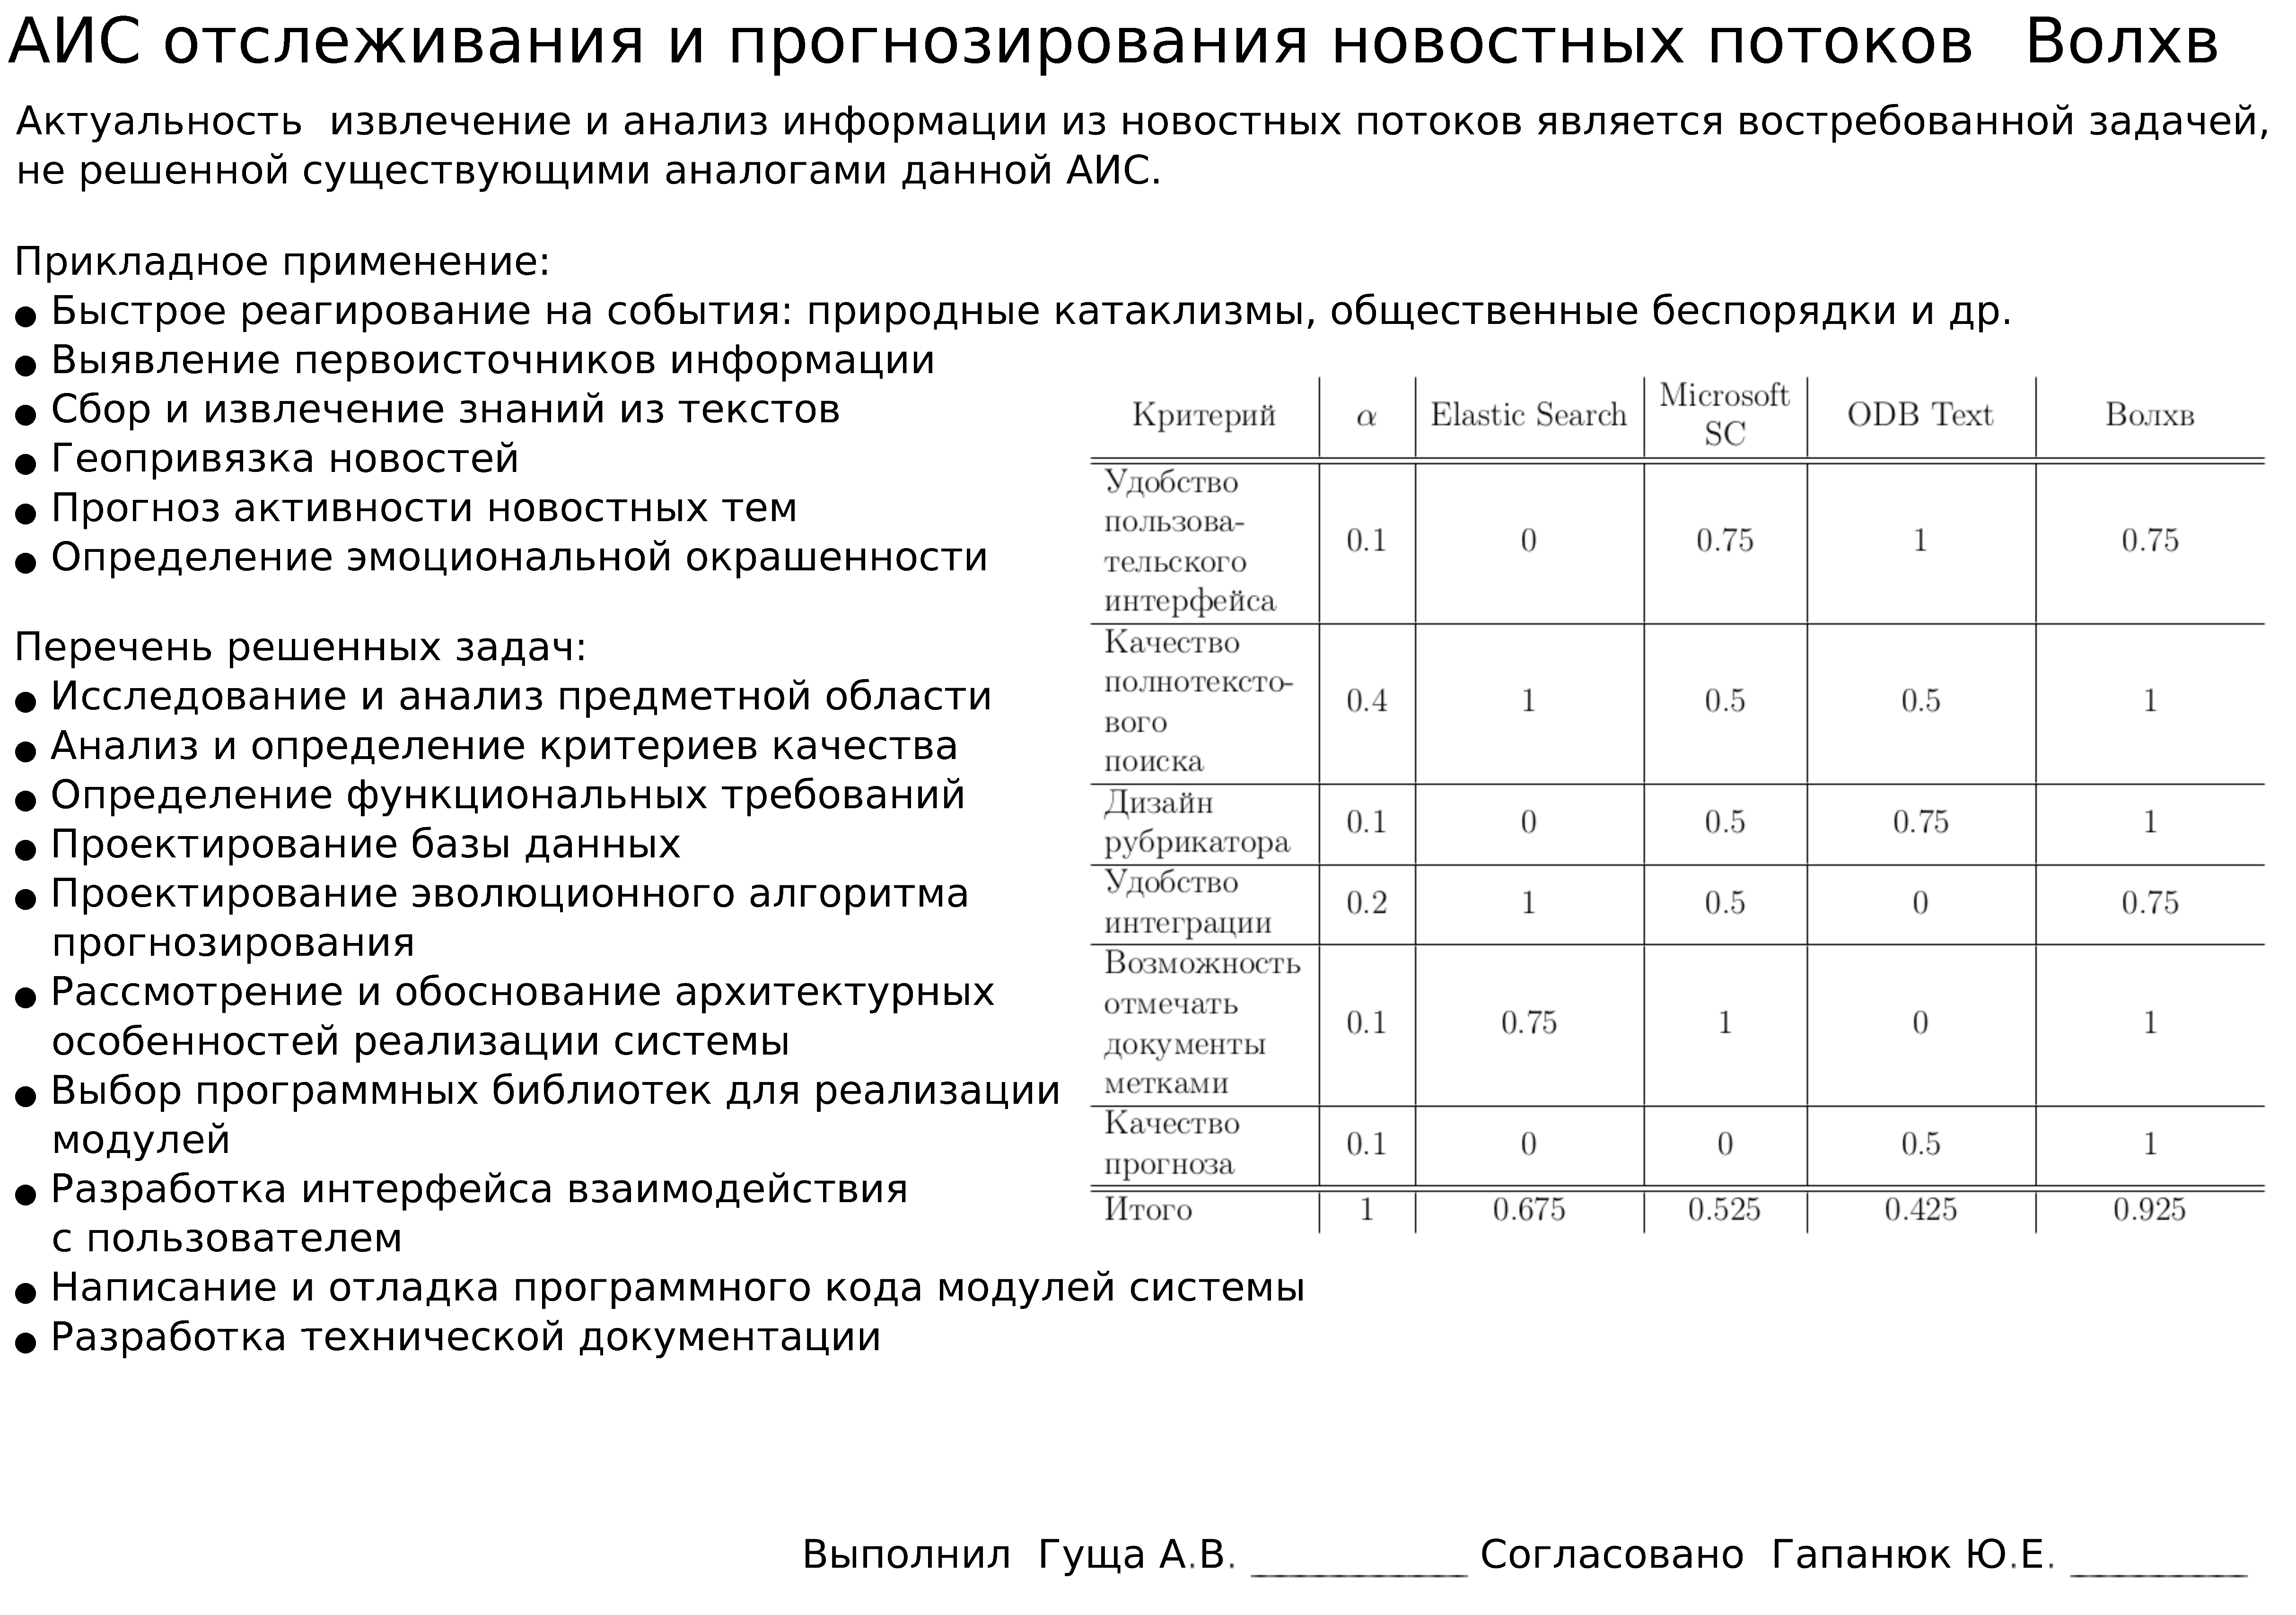
\includegraphics[width=0.90\textwidth]{lists/list1}
\end{ESKDdrawing}

\ESKDcolumnI{Схема предметной области}
\begin{ESKDdrawing}
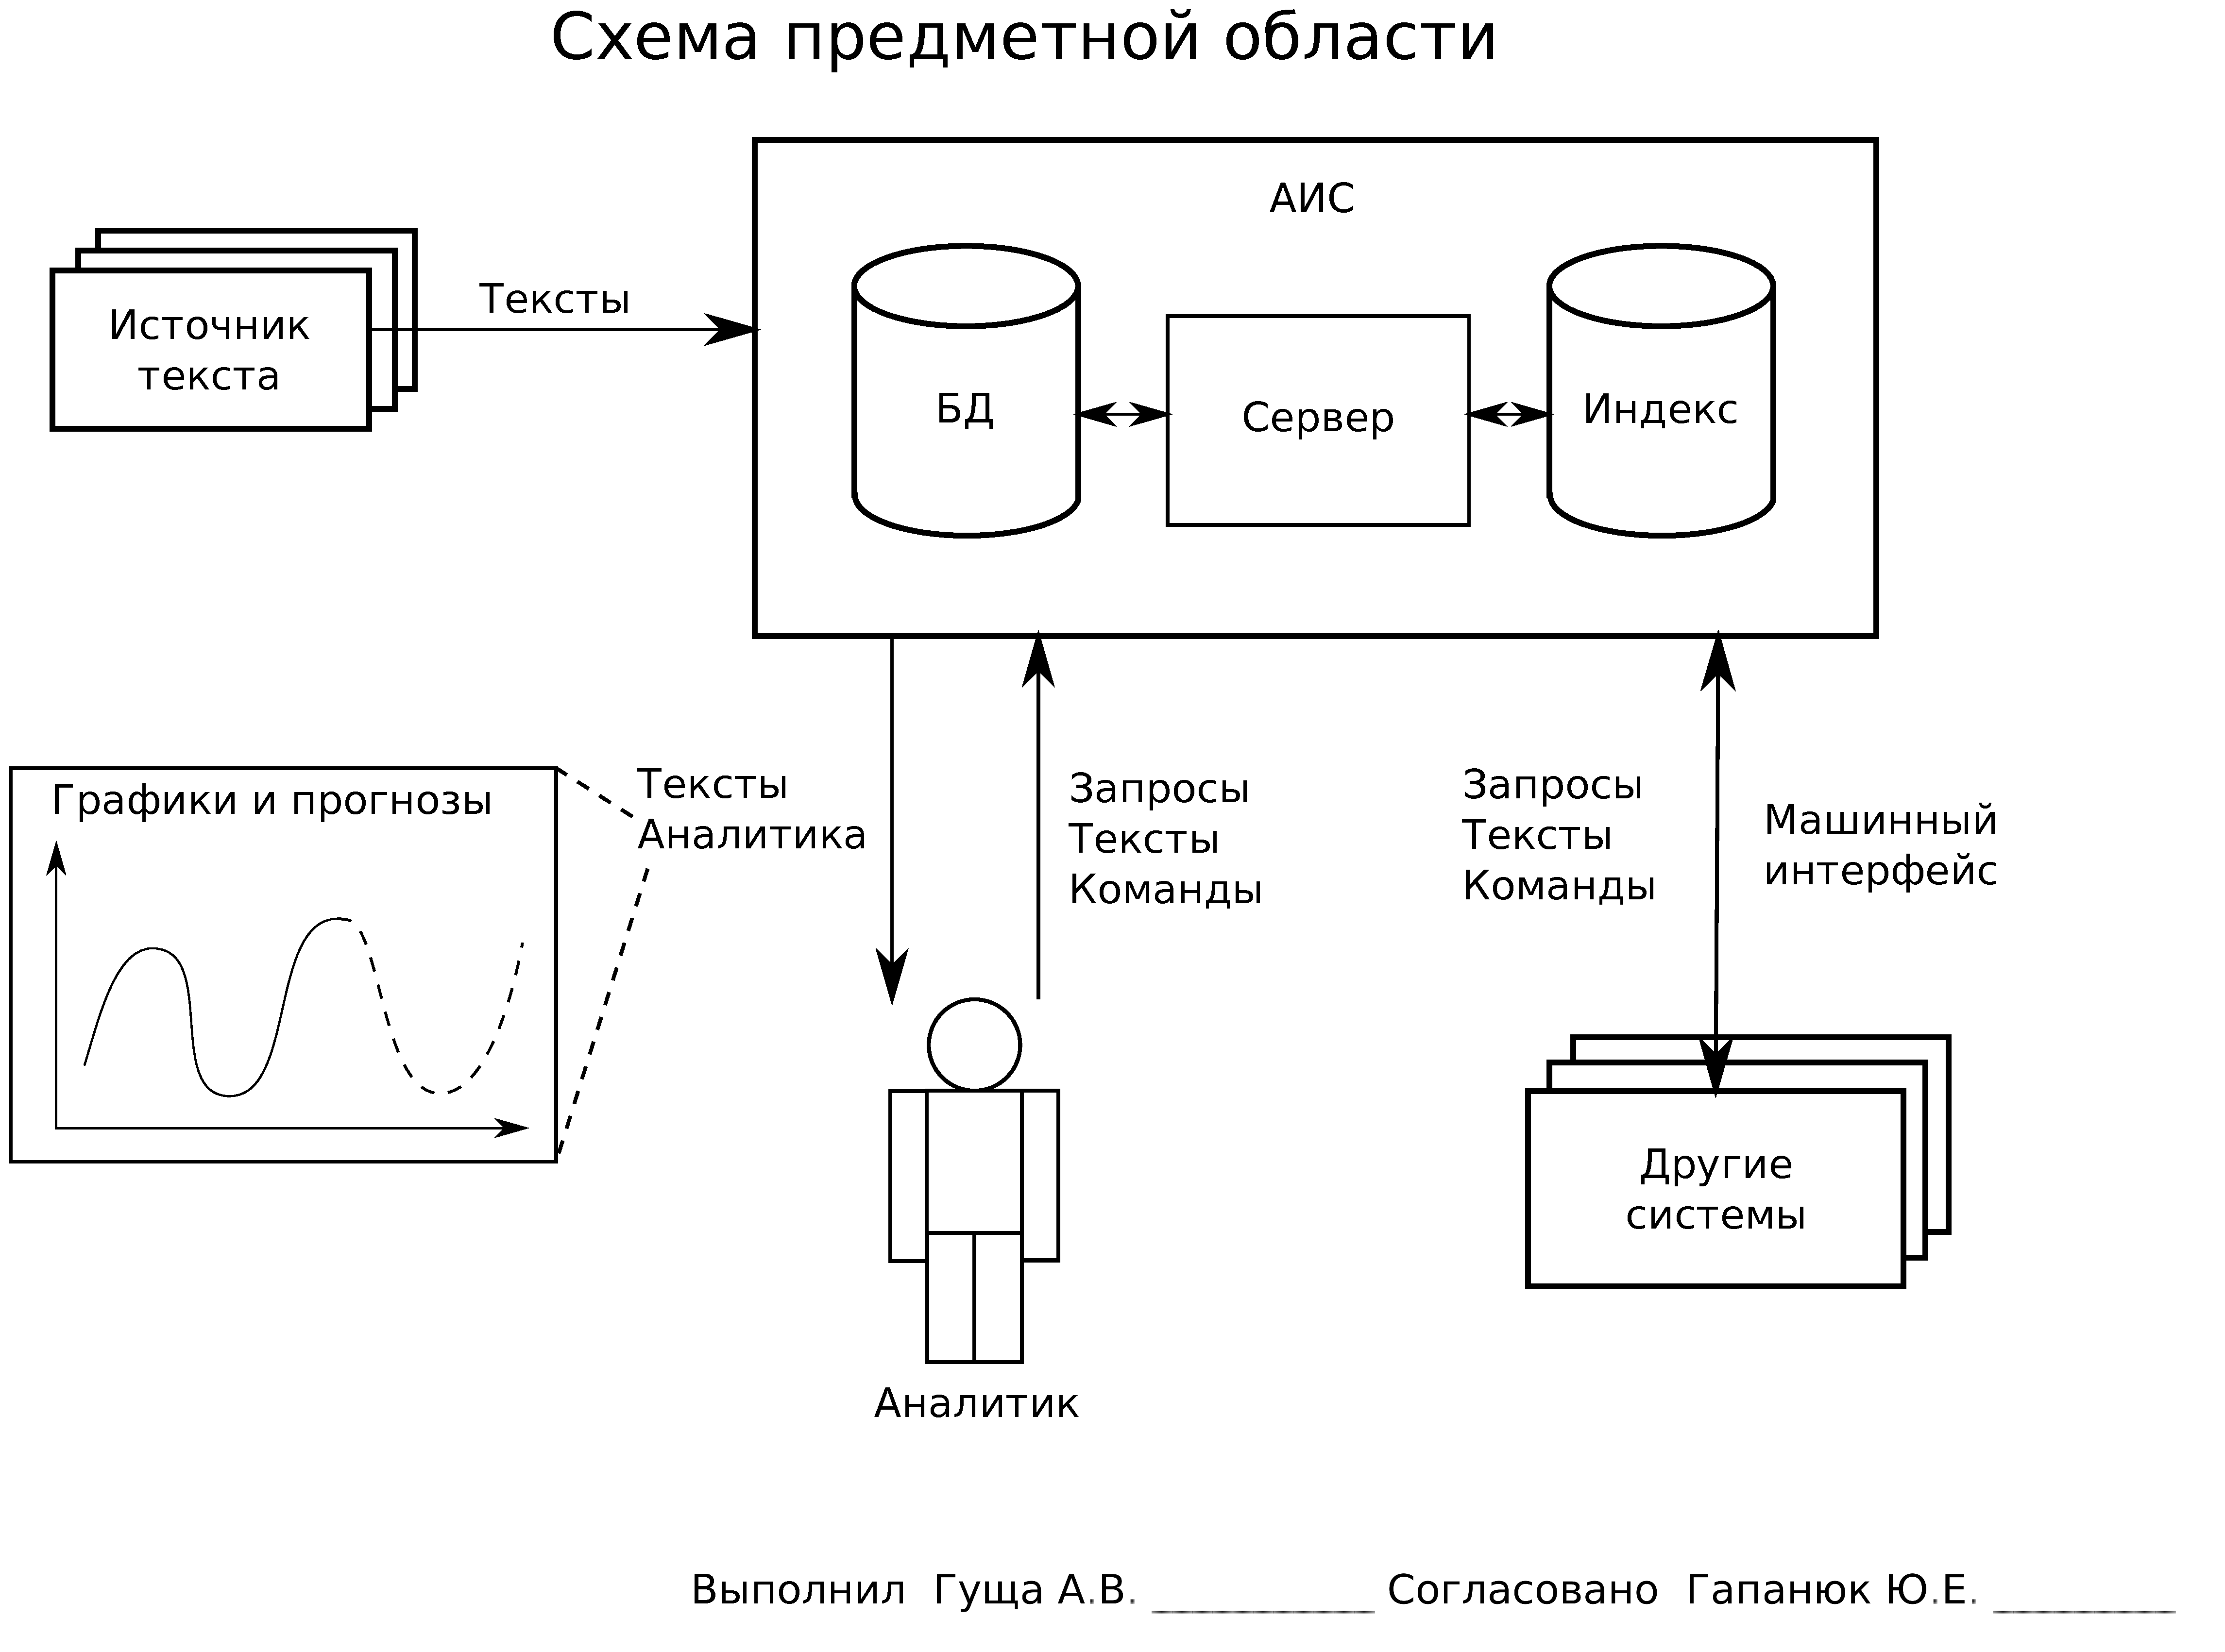
\includegraphics[width=0.90\textwidth]{lists/list2}
\end{ESKDdrawing}

\ESKDcolumnI{Бизнес процесс АИС}
\begin{ESKDdrawing}
\centering
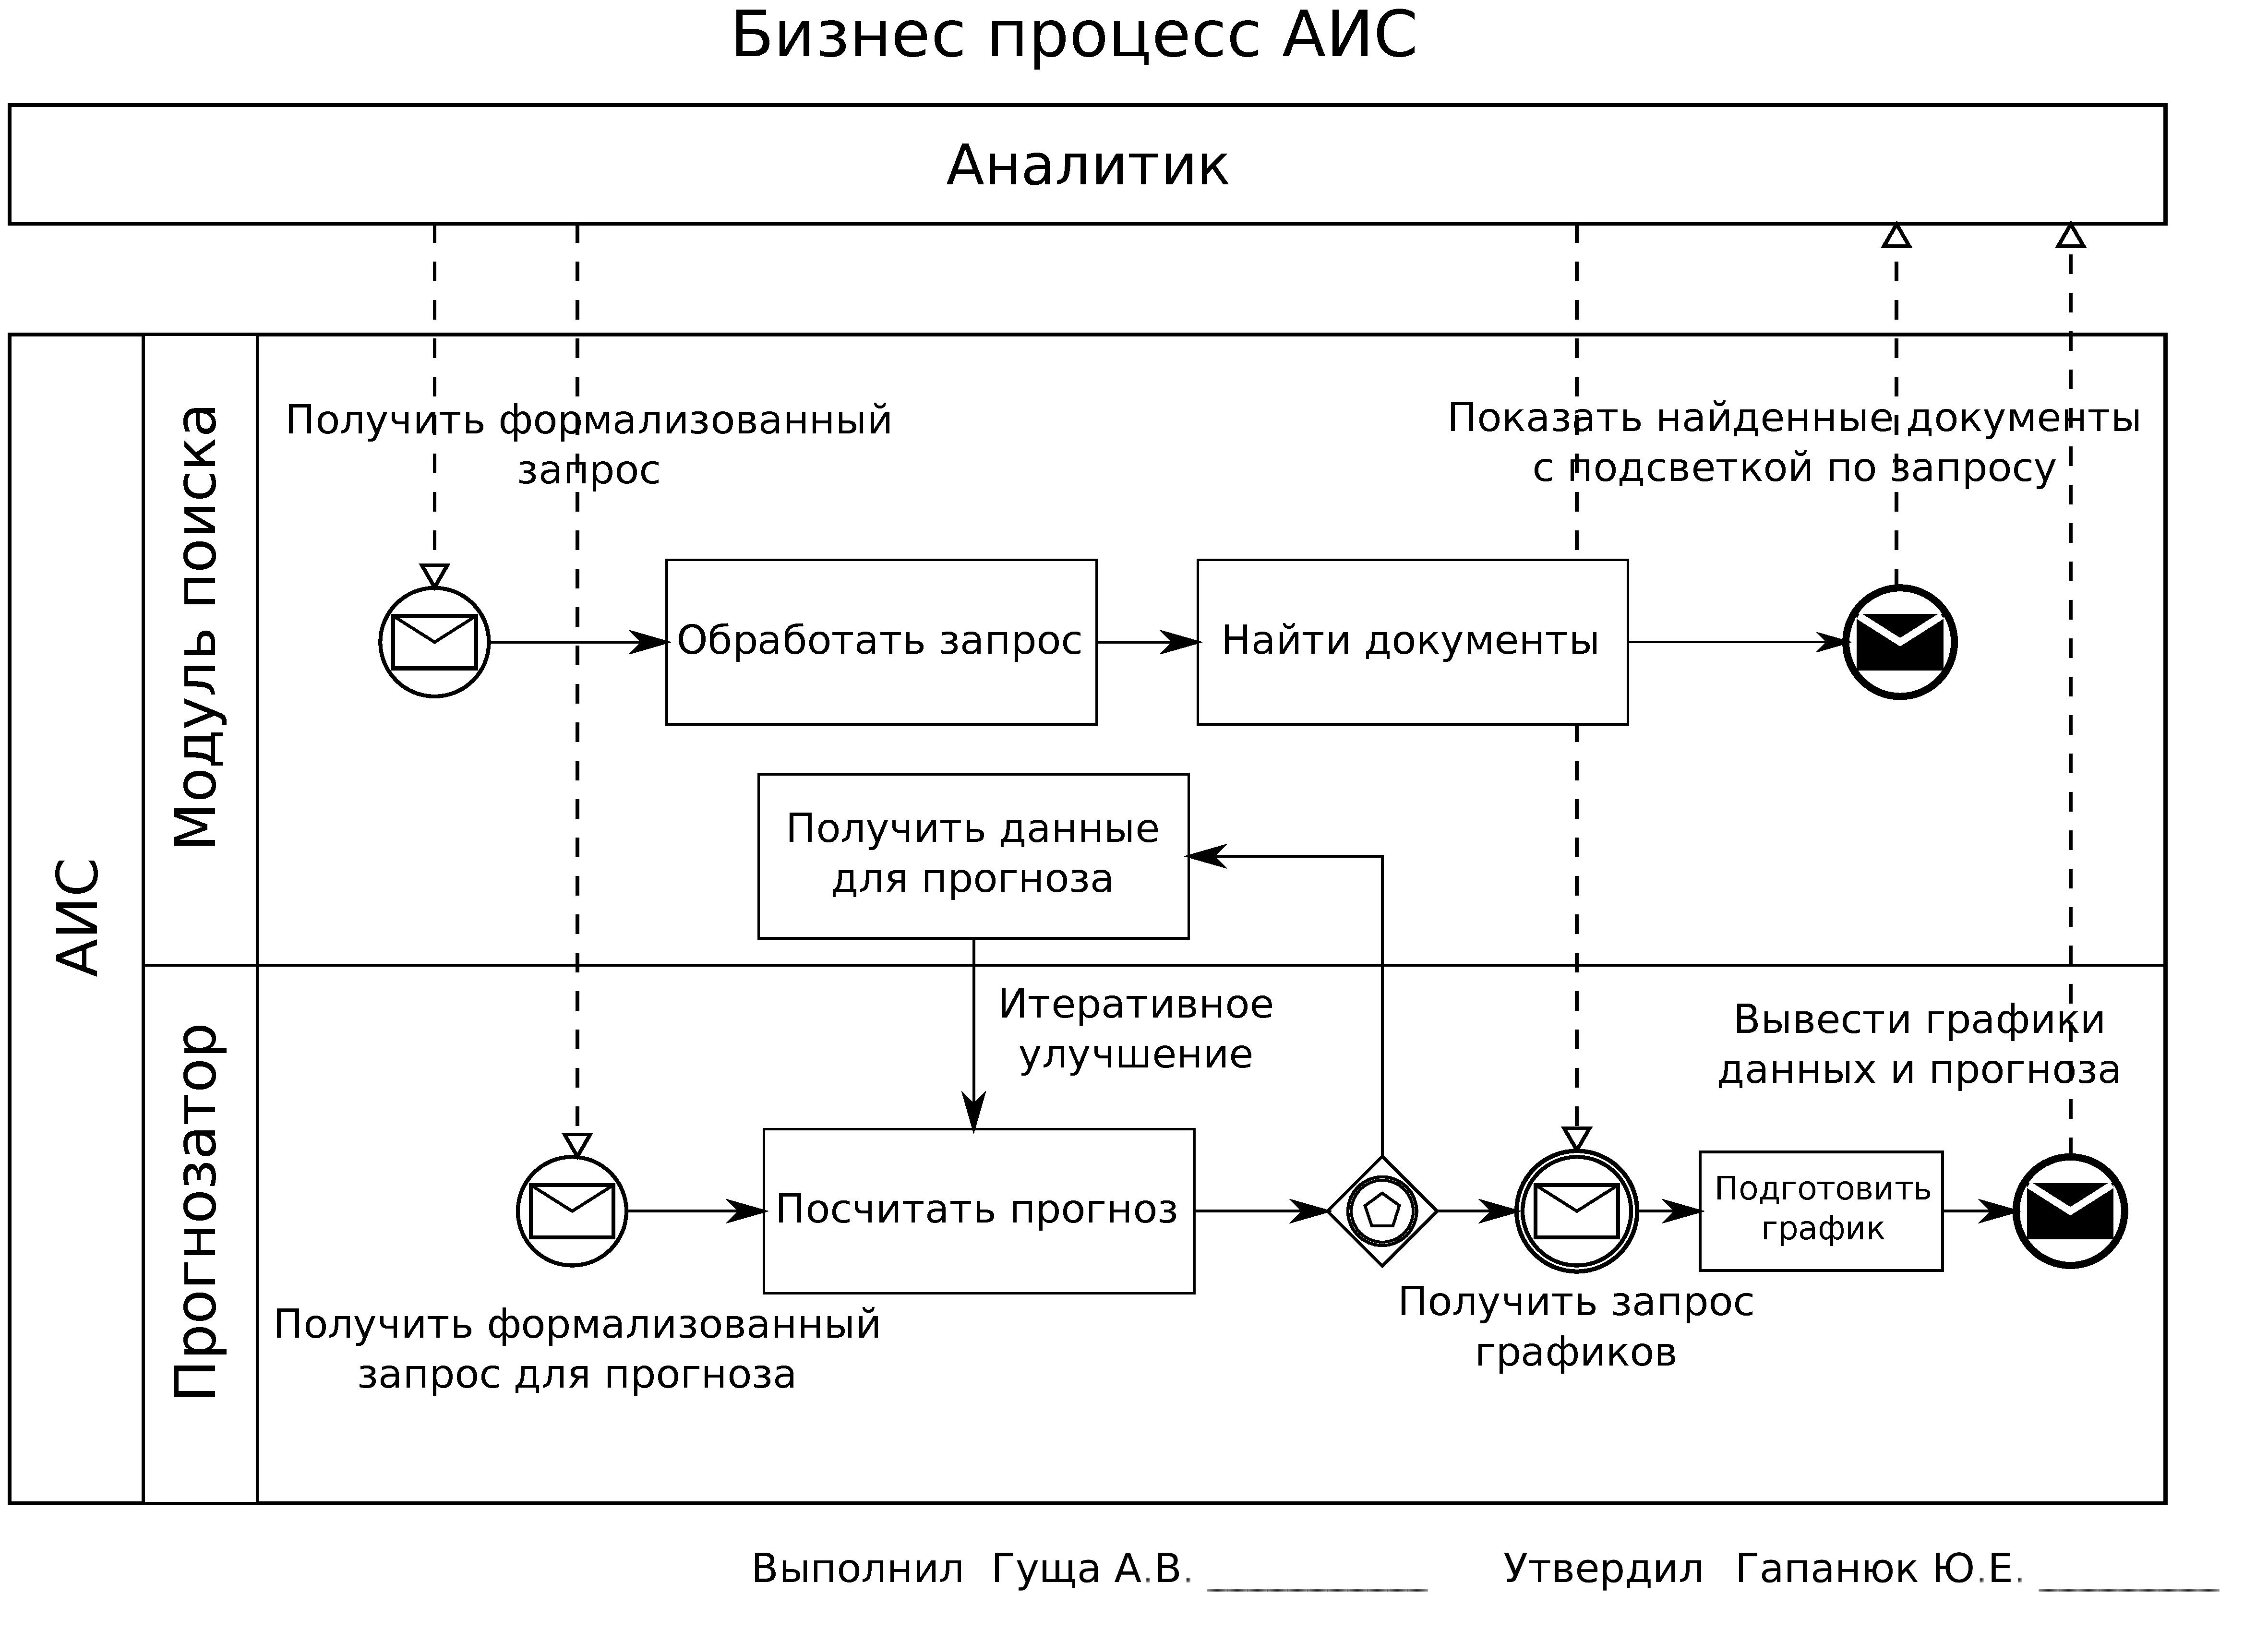
\includegraphics[width=0.90\textwidth]{lists/list12}
\end{ESKDdrawing}

\ESKDcolumnI{Структурная схема}
\begin{ESKDdrawing}
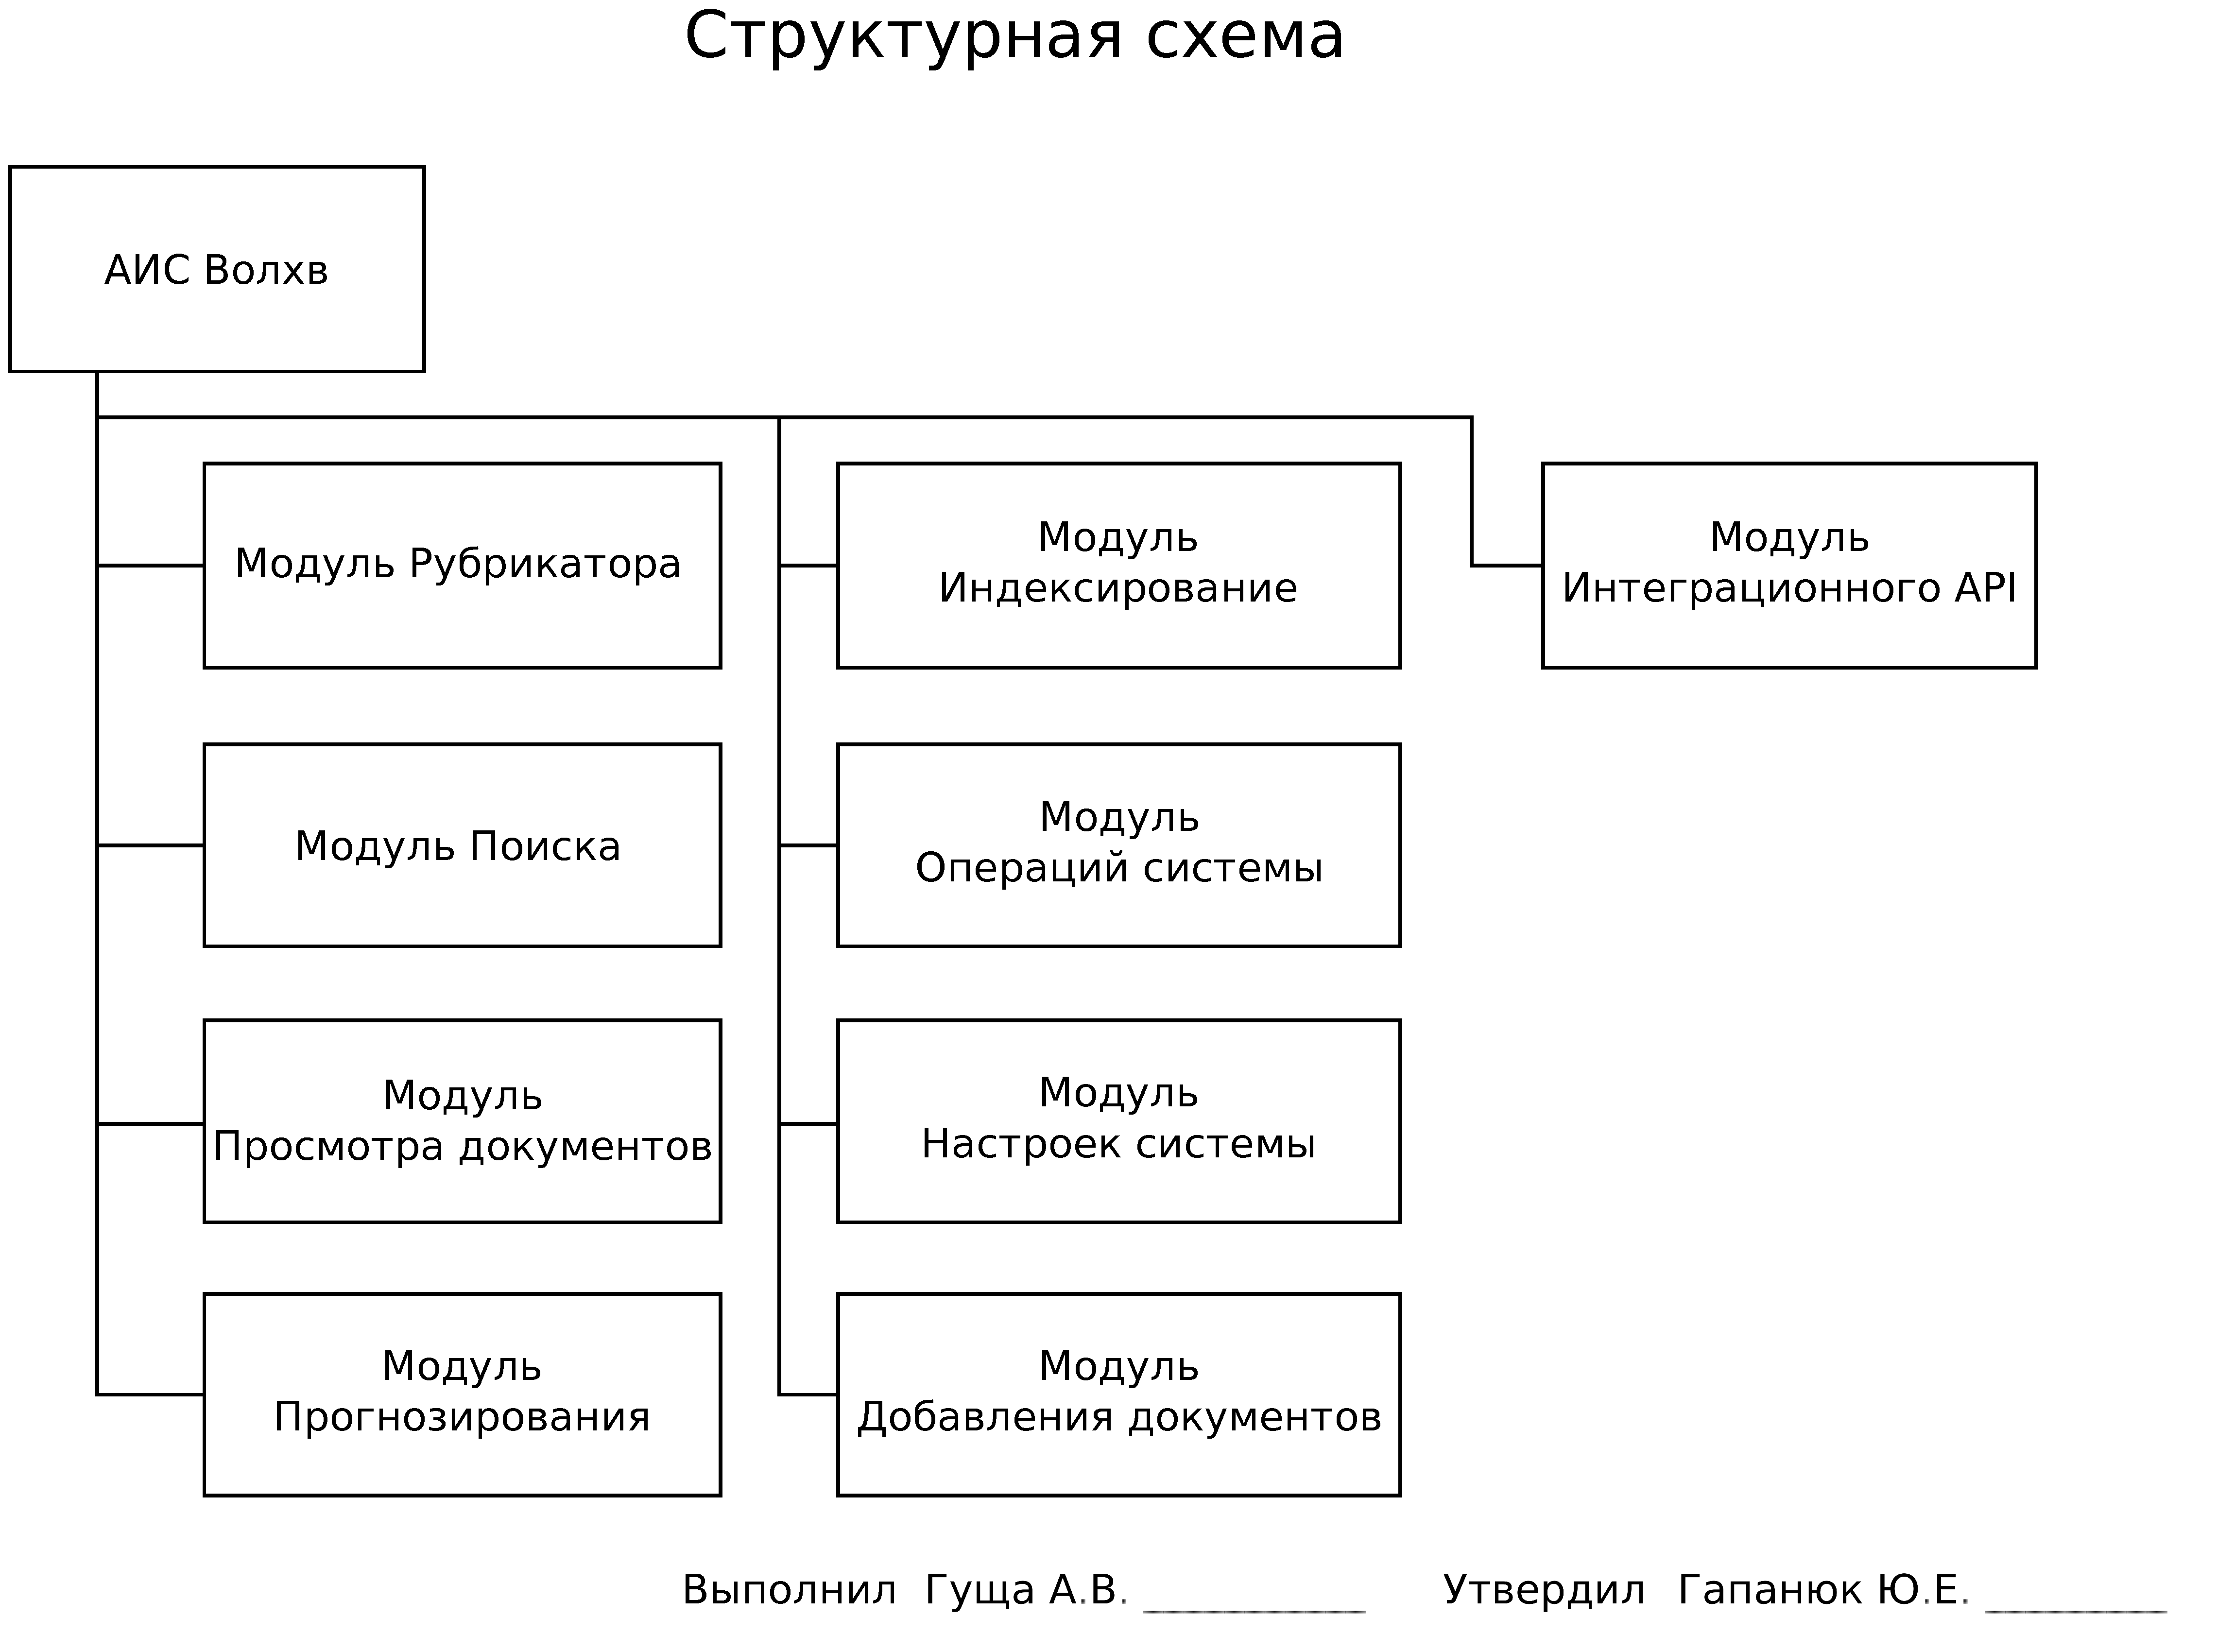
\includegraphics[width=0.90\textwidth]{lists/list3}
\end{ESKDdrawing}

\ESKDcolumnI{Технологические модули системы}
\begin{ESKDdrawing}
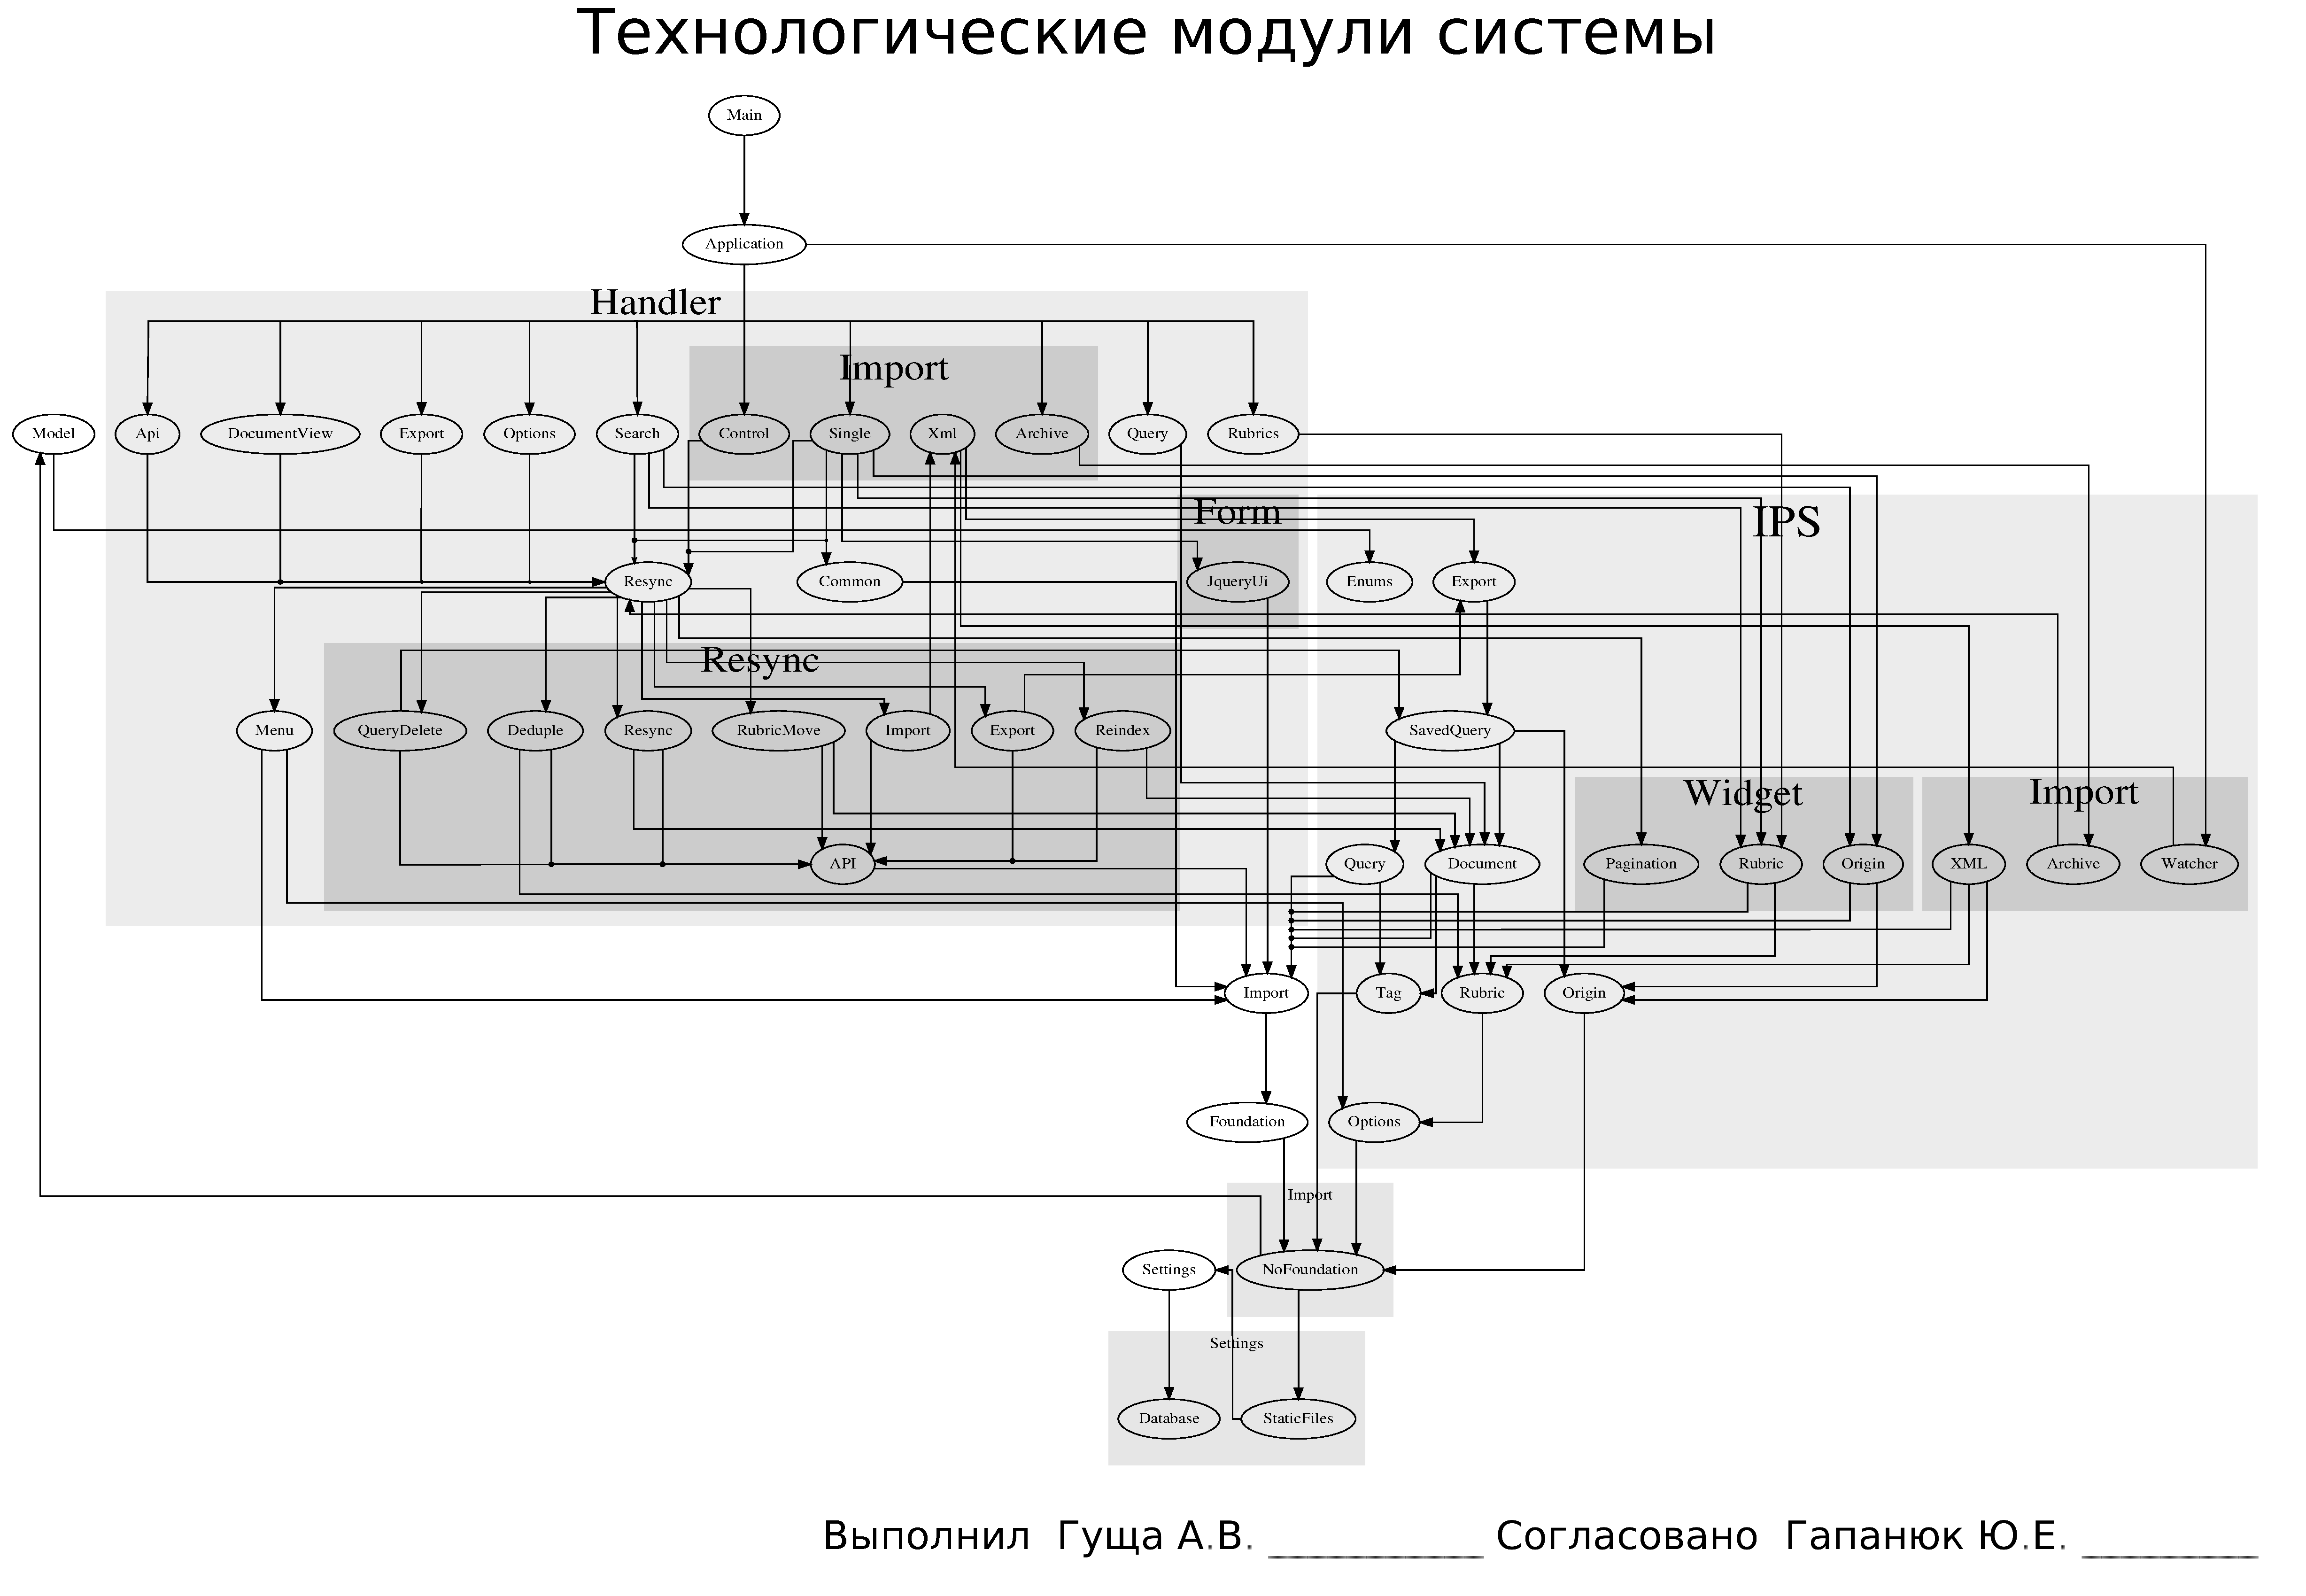
\includegraphics[width=0.90\textwidth]{lists/list4}
\end{ESKDdrawing}

\ESKDcolumnI{Инфологическая модель БД}
\begin{ESKDdrawing}
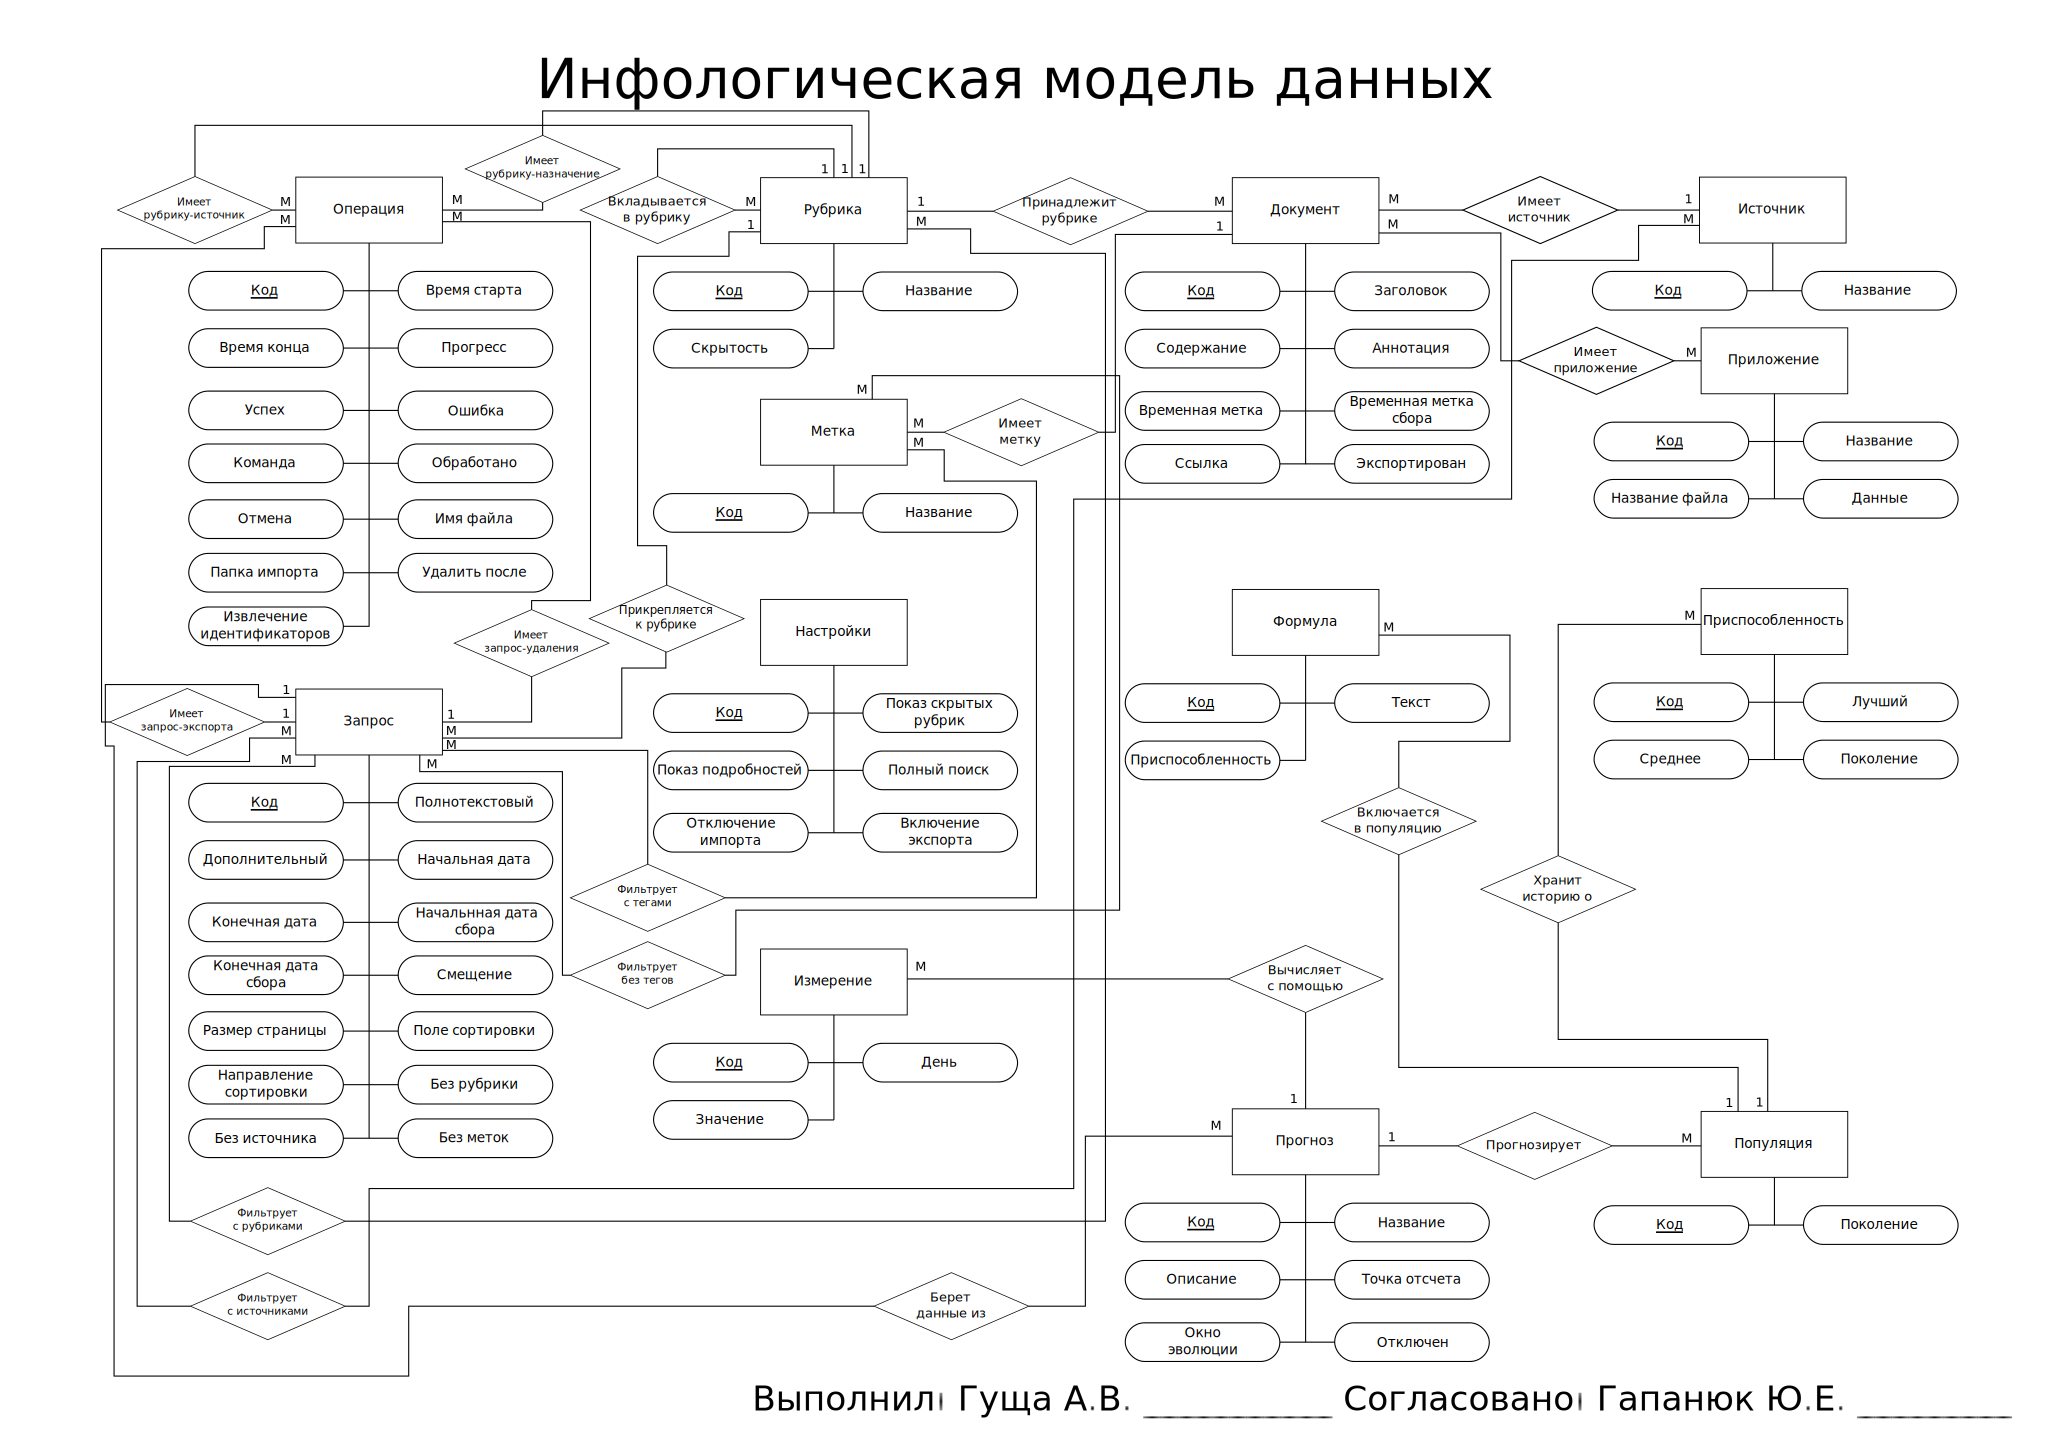
\includegraphics[width=0.90\textwidth]{lists/list5}
\end{ESKDdrawing}

\ESKDcolumnI{Даталогическая модель БД}
\begin{ESKDdrawing}
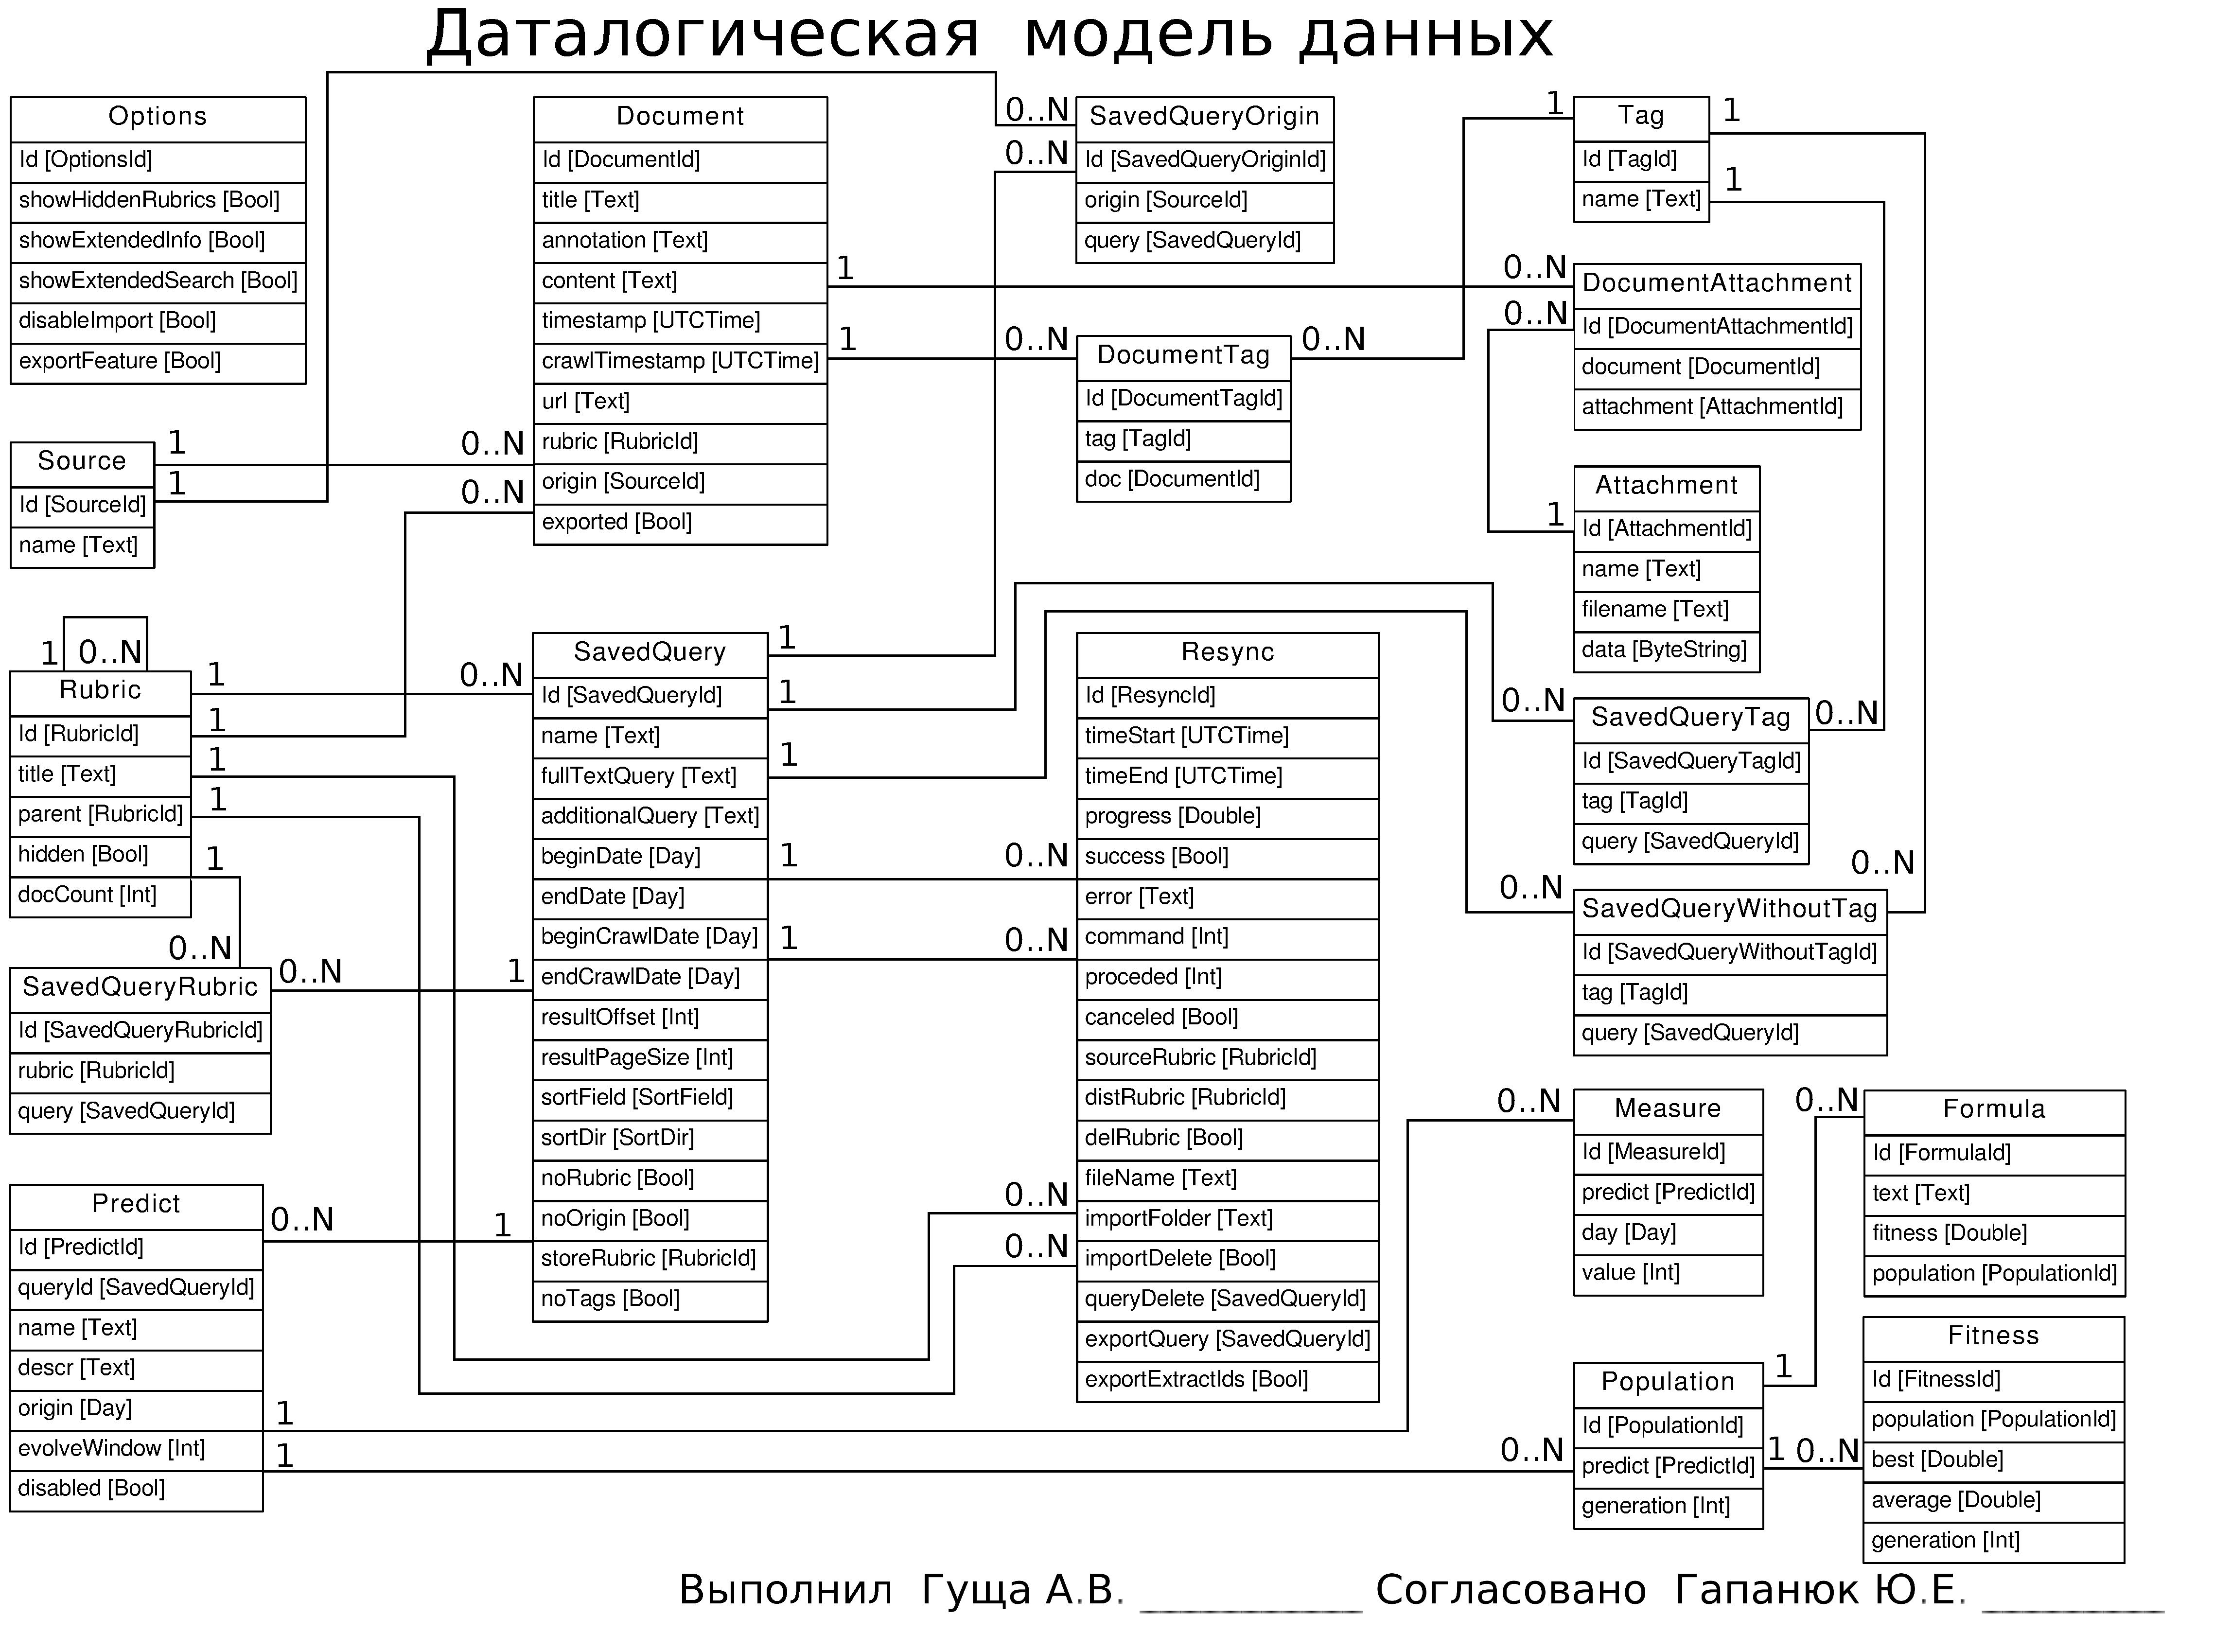
\includegraphics[width=0.90\textwidth]{lists/list6}
\end{ESKDdrawing}

\ESKDcolumnI{Диаграмма типов}
\begin{ESKDdrawing}

\includegraphics[width=0.90\textwidth]{lists/list7}
\end{ESKDdrawing}

\ESKDcolumnI{Граф диалога с пользователем}
\begin{ESKDdrawing}
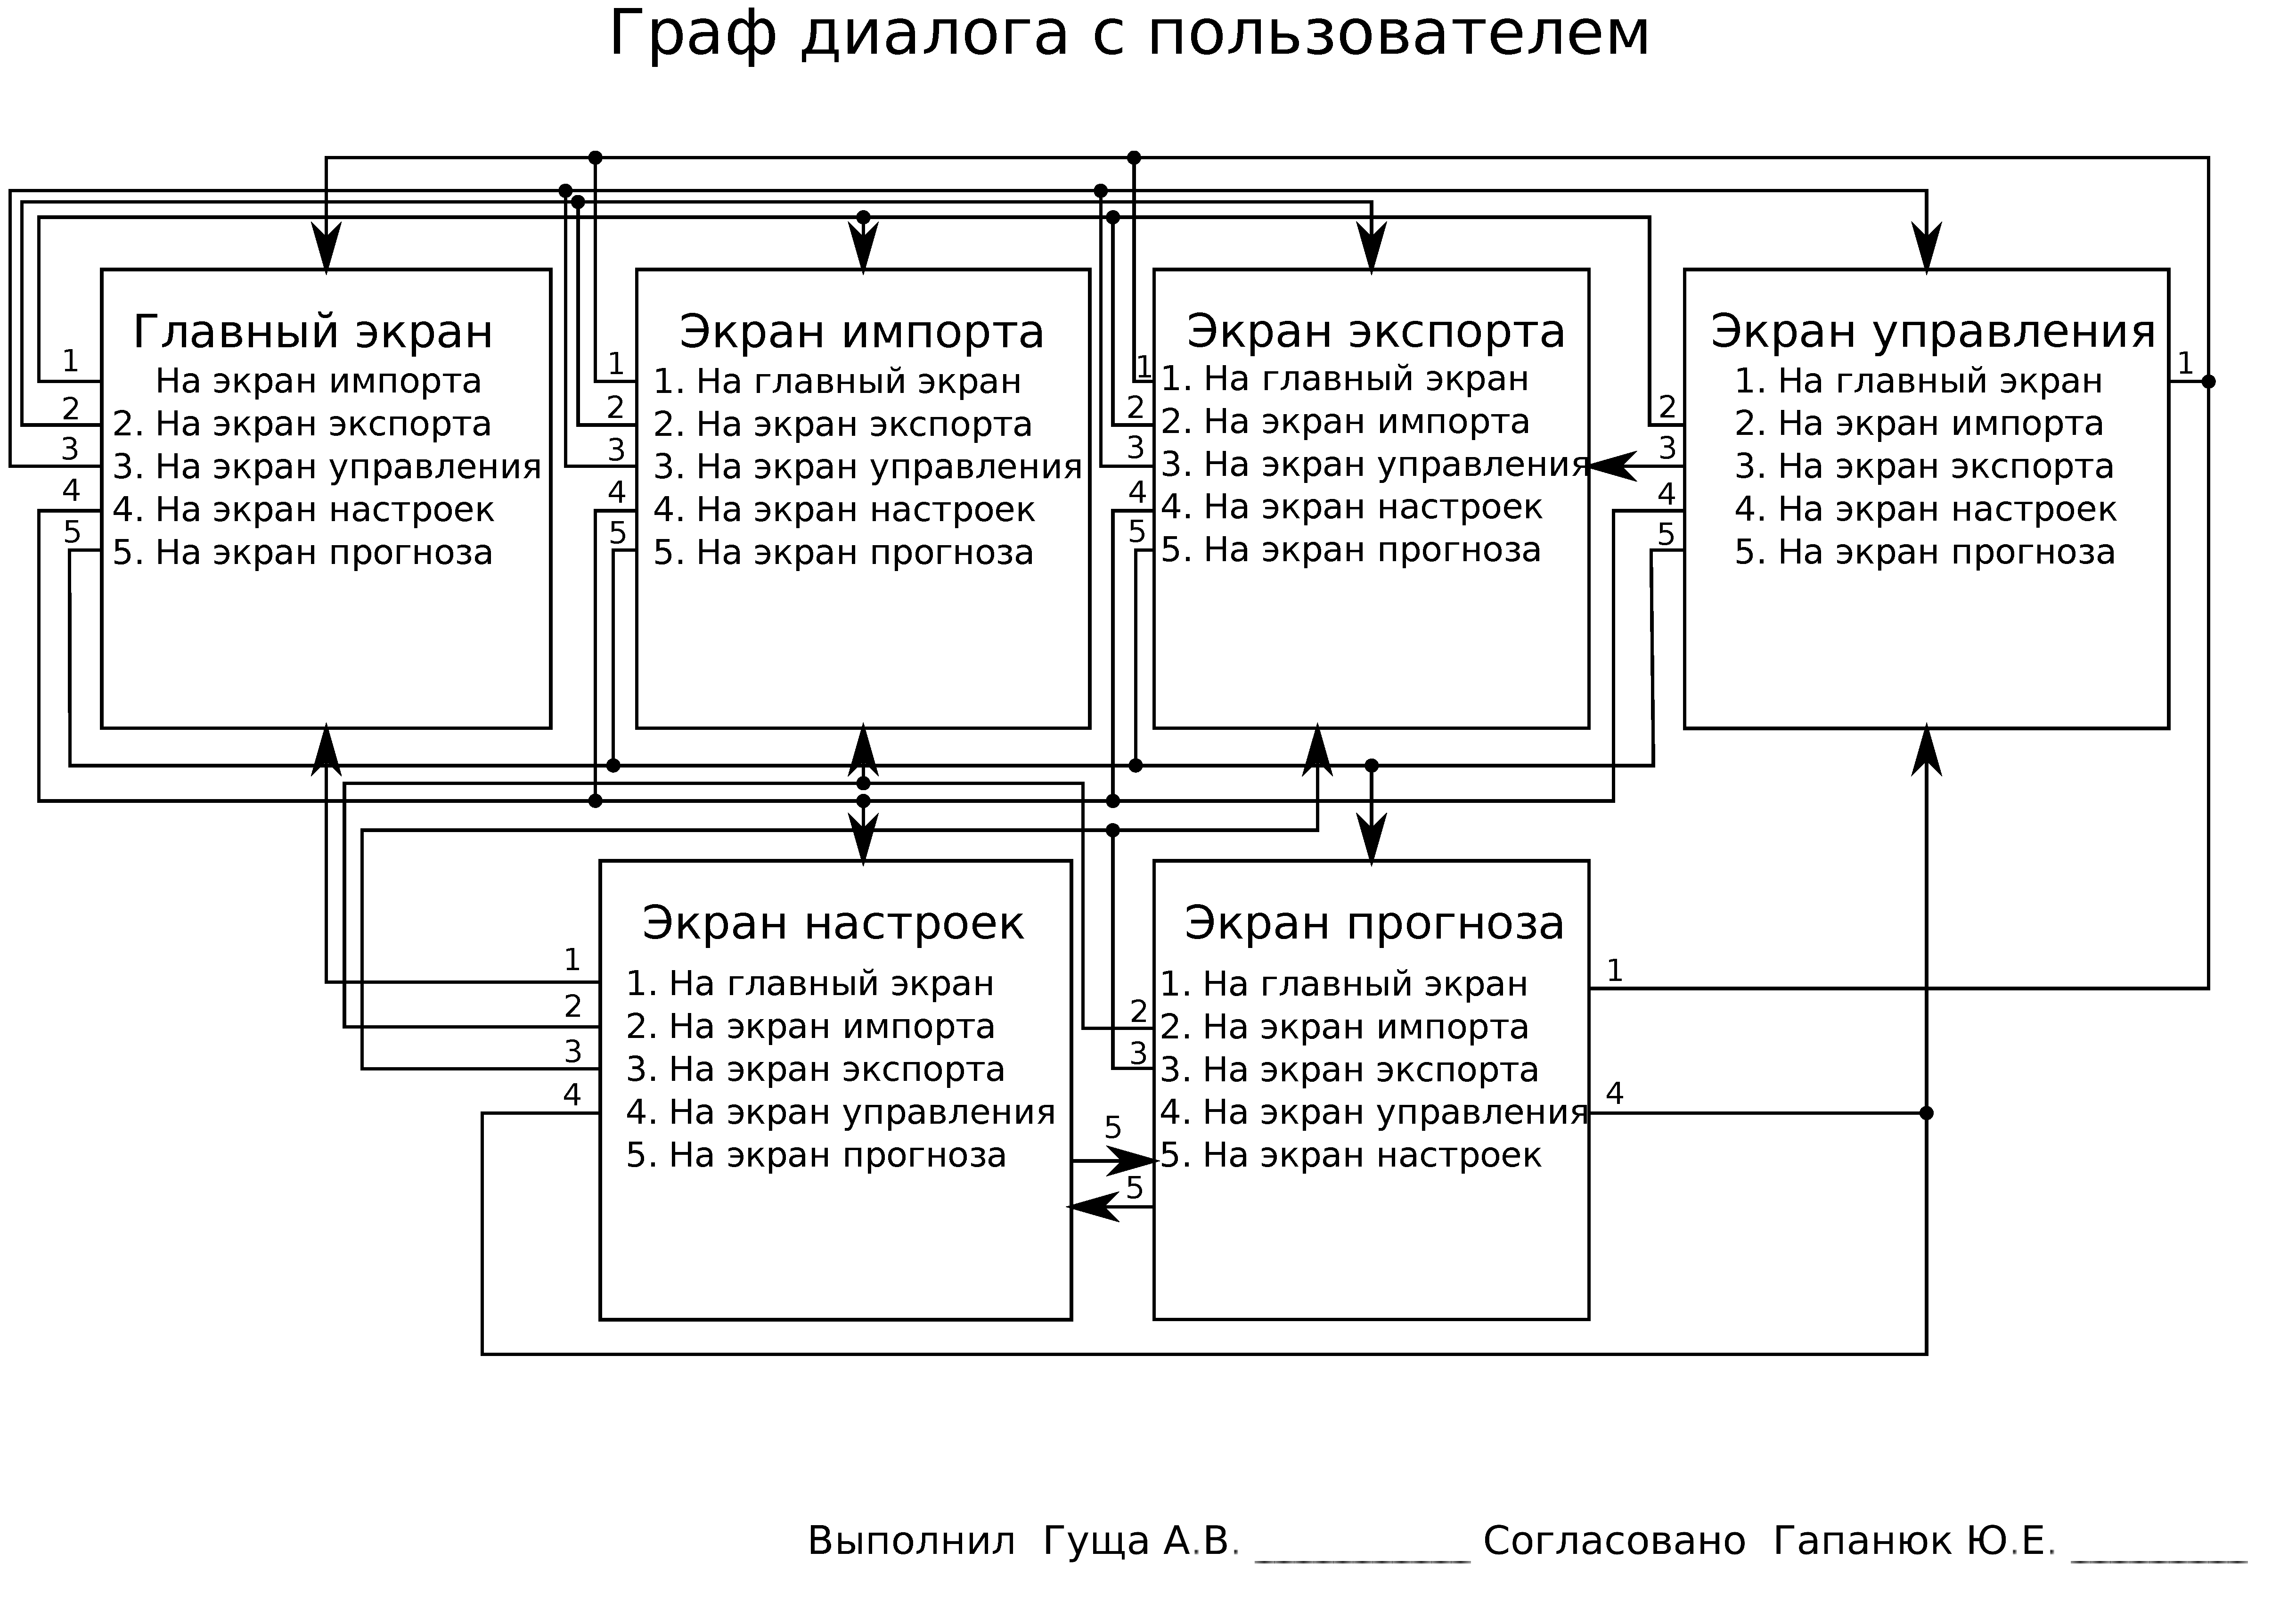
\includegraphics[width=0.90\textwidth]{lists/list8}
\end{ESKDdrawing}

\ESKDcolumnI{Основные экранные формы}
\begin{ESKDdrawing}
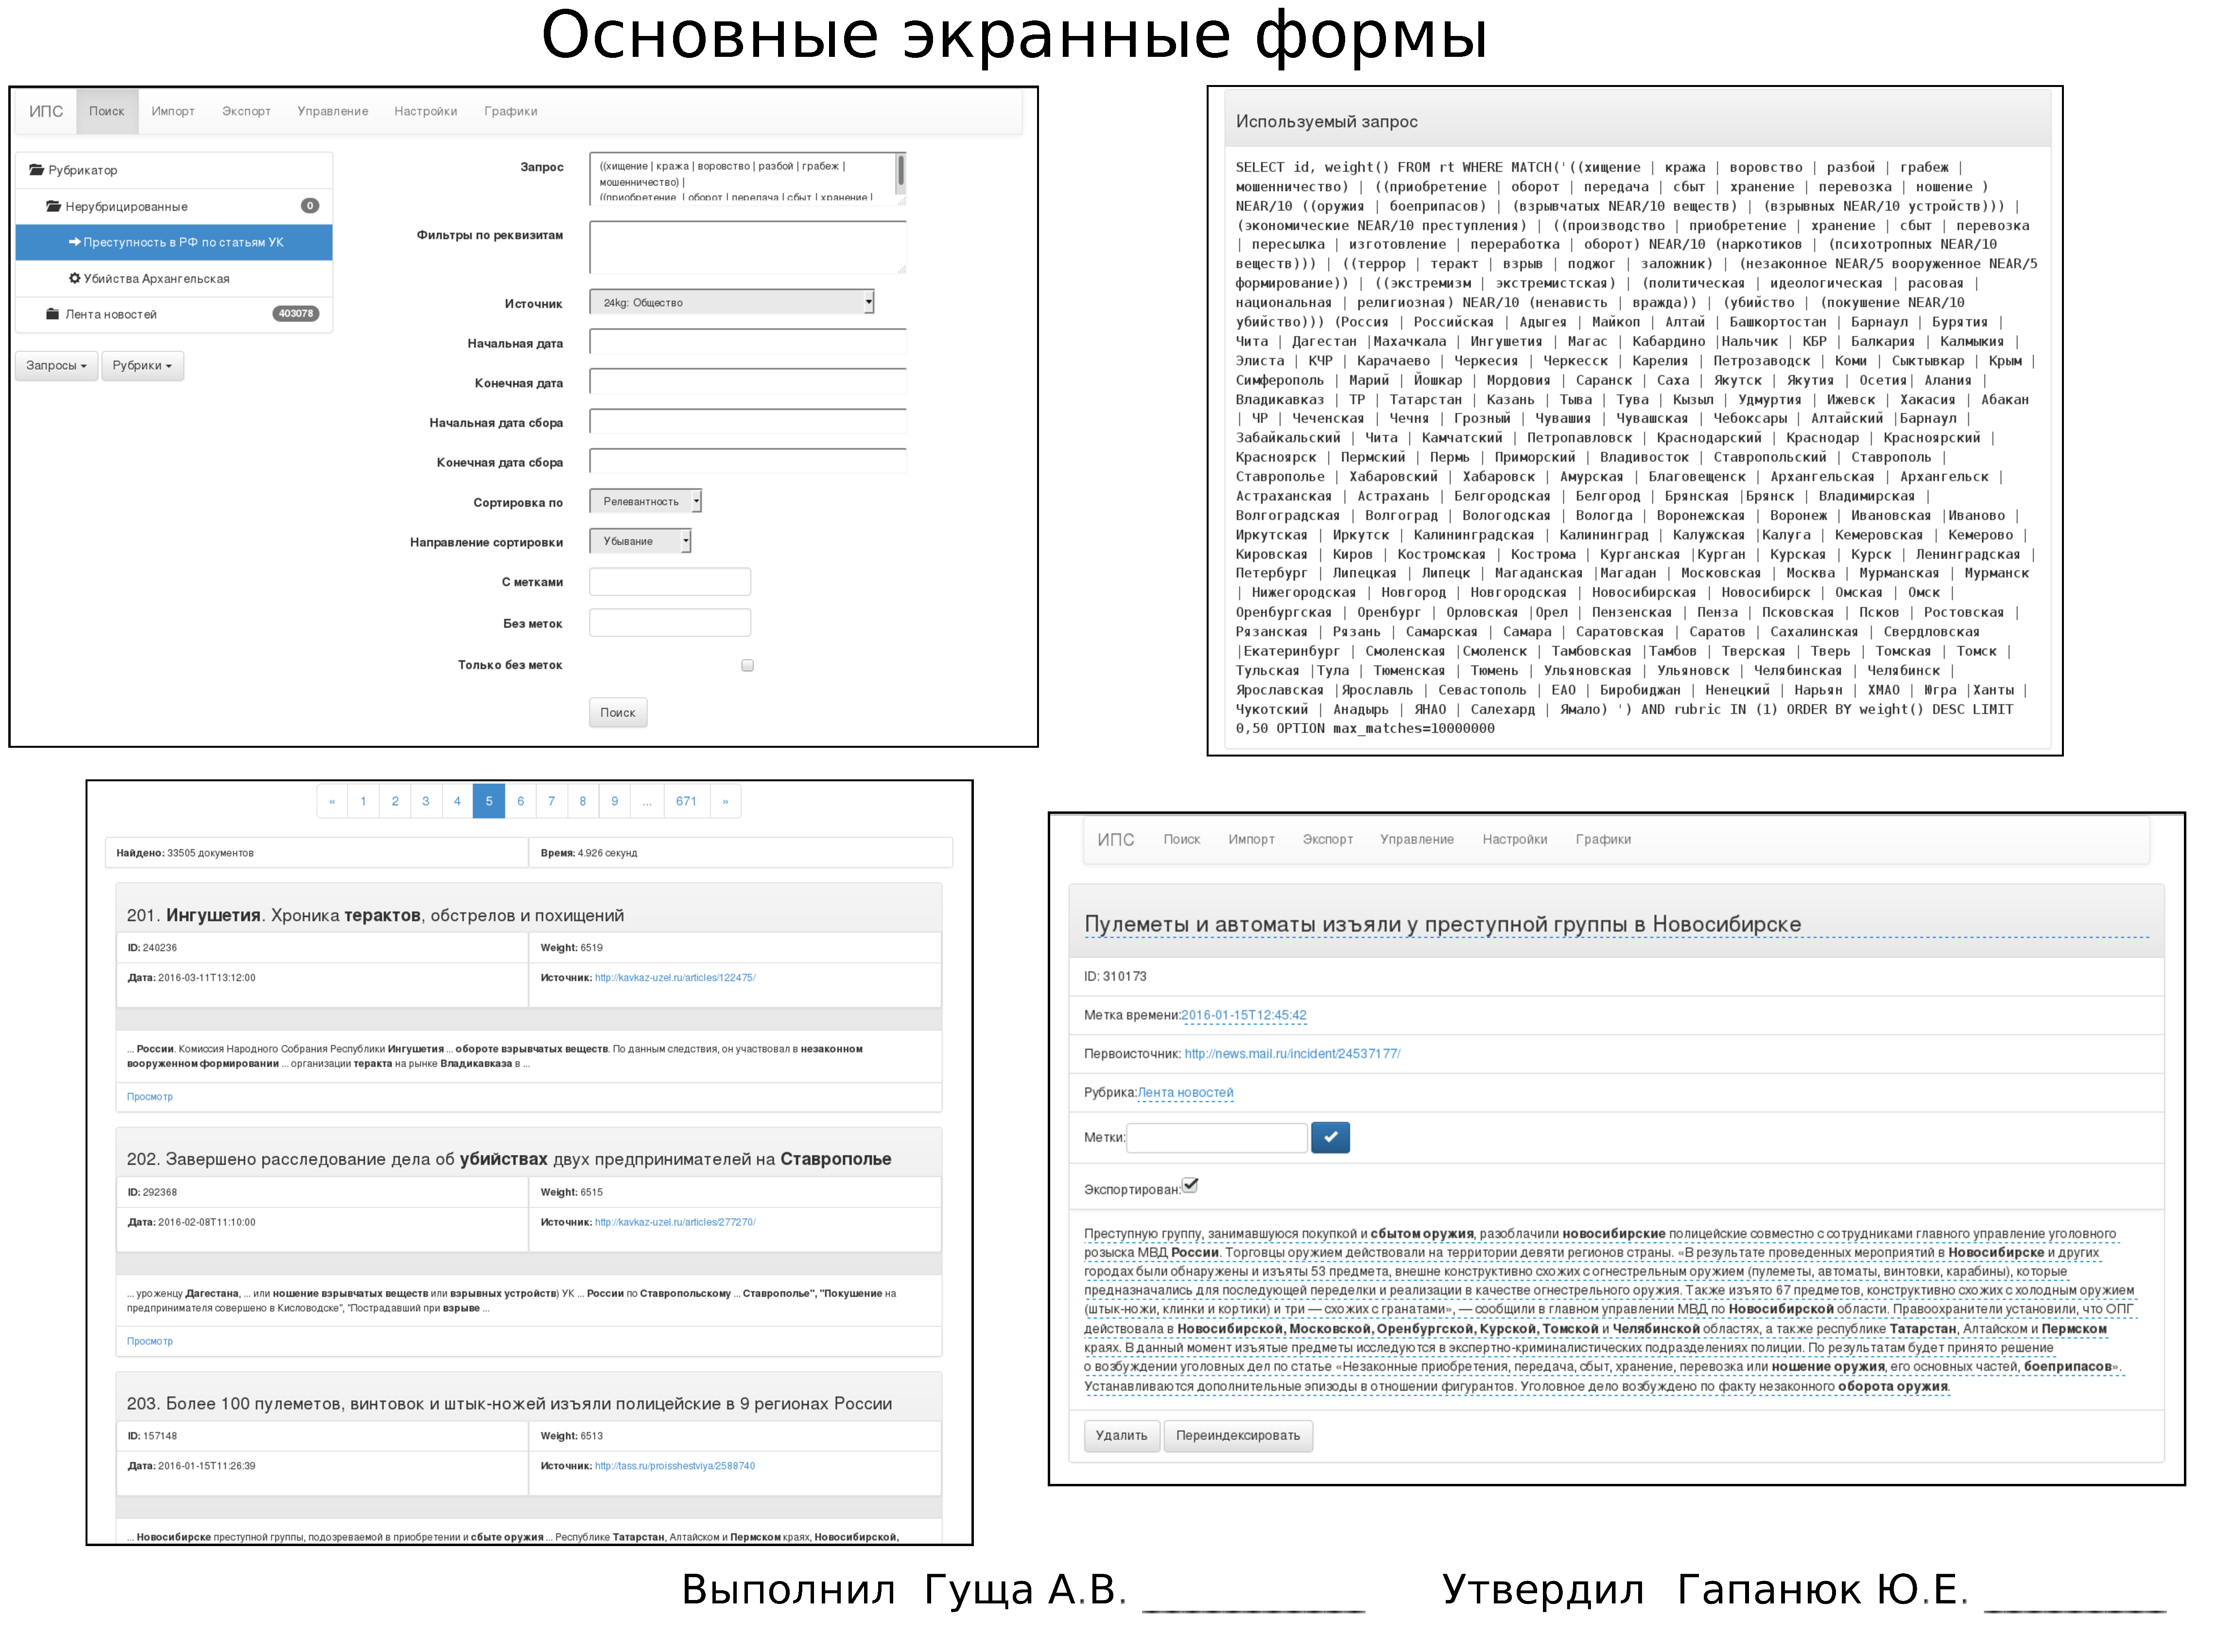
\includegraphics[width=0.90\textwidth]{lists/list9_1}
\end{ESKDdrawing}

\ESKDcolumnI{Основные экранные формы}
\begin{ESKDdrawing}
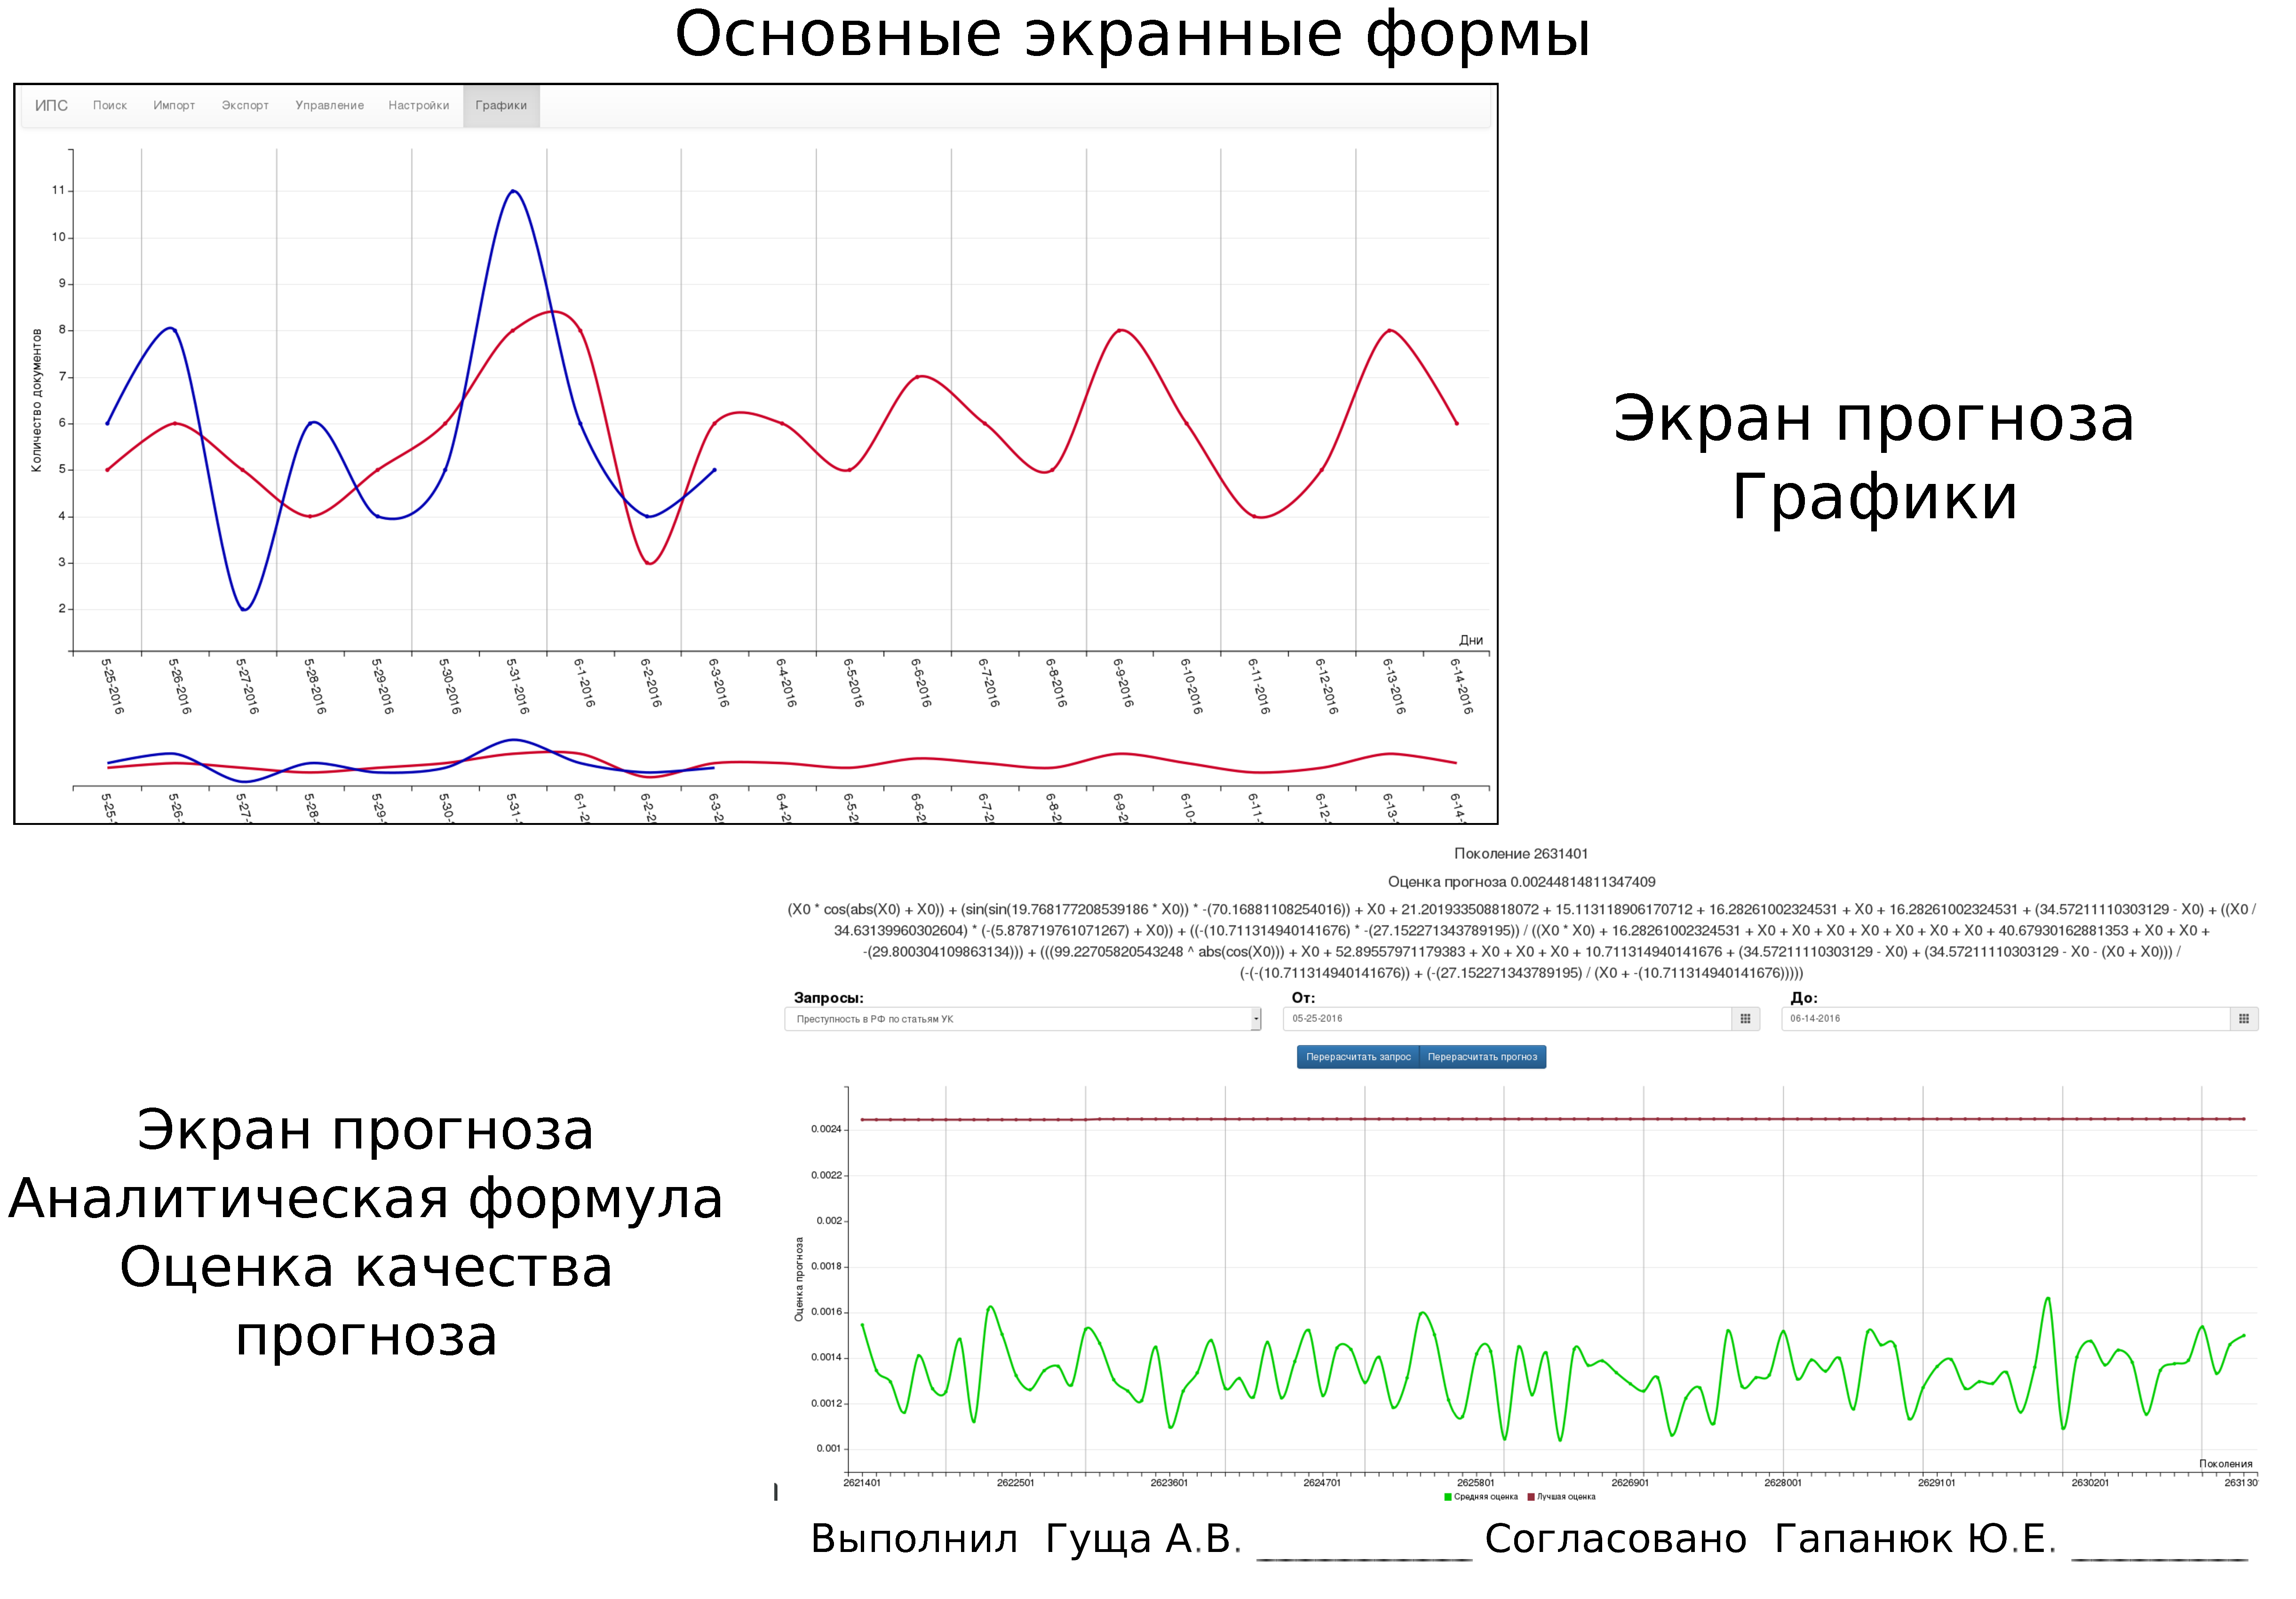
\includegraphics[width=0.90\textwidth]{lists/list9_2}
\end{ESKDdrawing}


\ESKDcolumnI{Исследовательская часть}
\begin{ESKDdrawing}
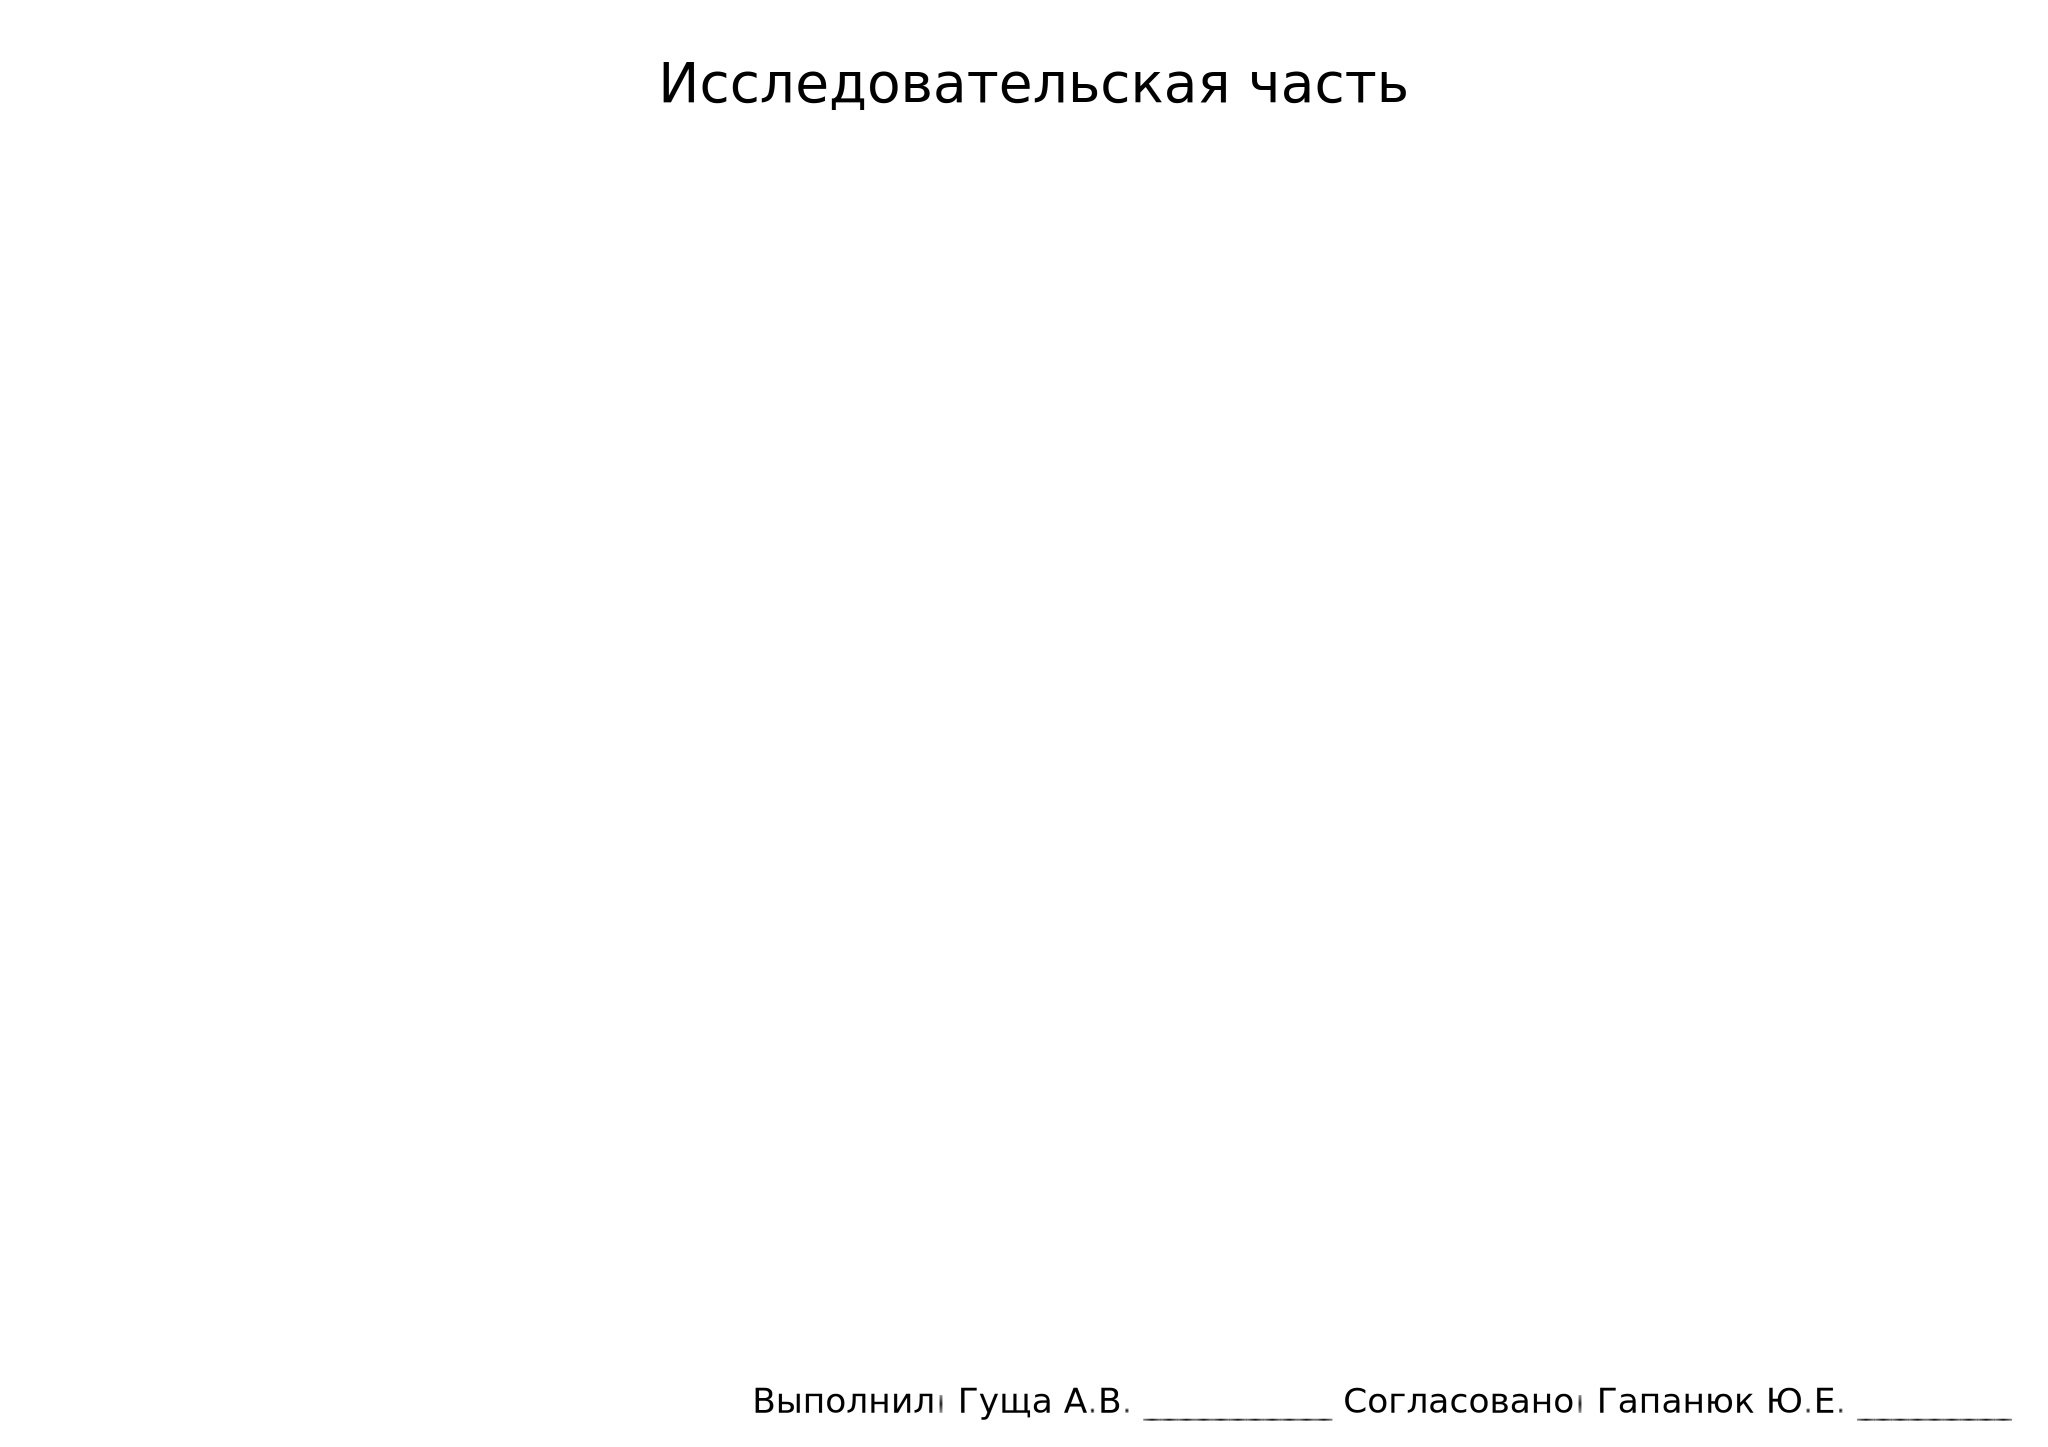
\includegraphics[width=0.90\textwidth]{lists/list10_1}
\end{ESKDdrawing}

\ESKDcolumnI{Исследовательская часть}
\begin{ESKDdrawing}
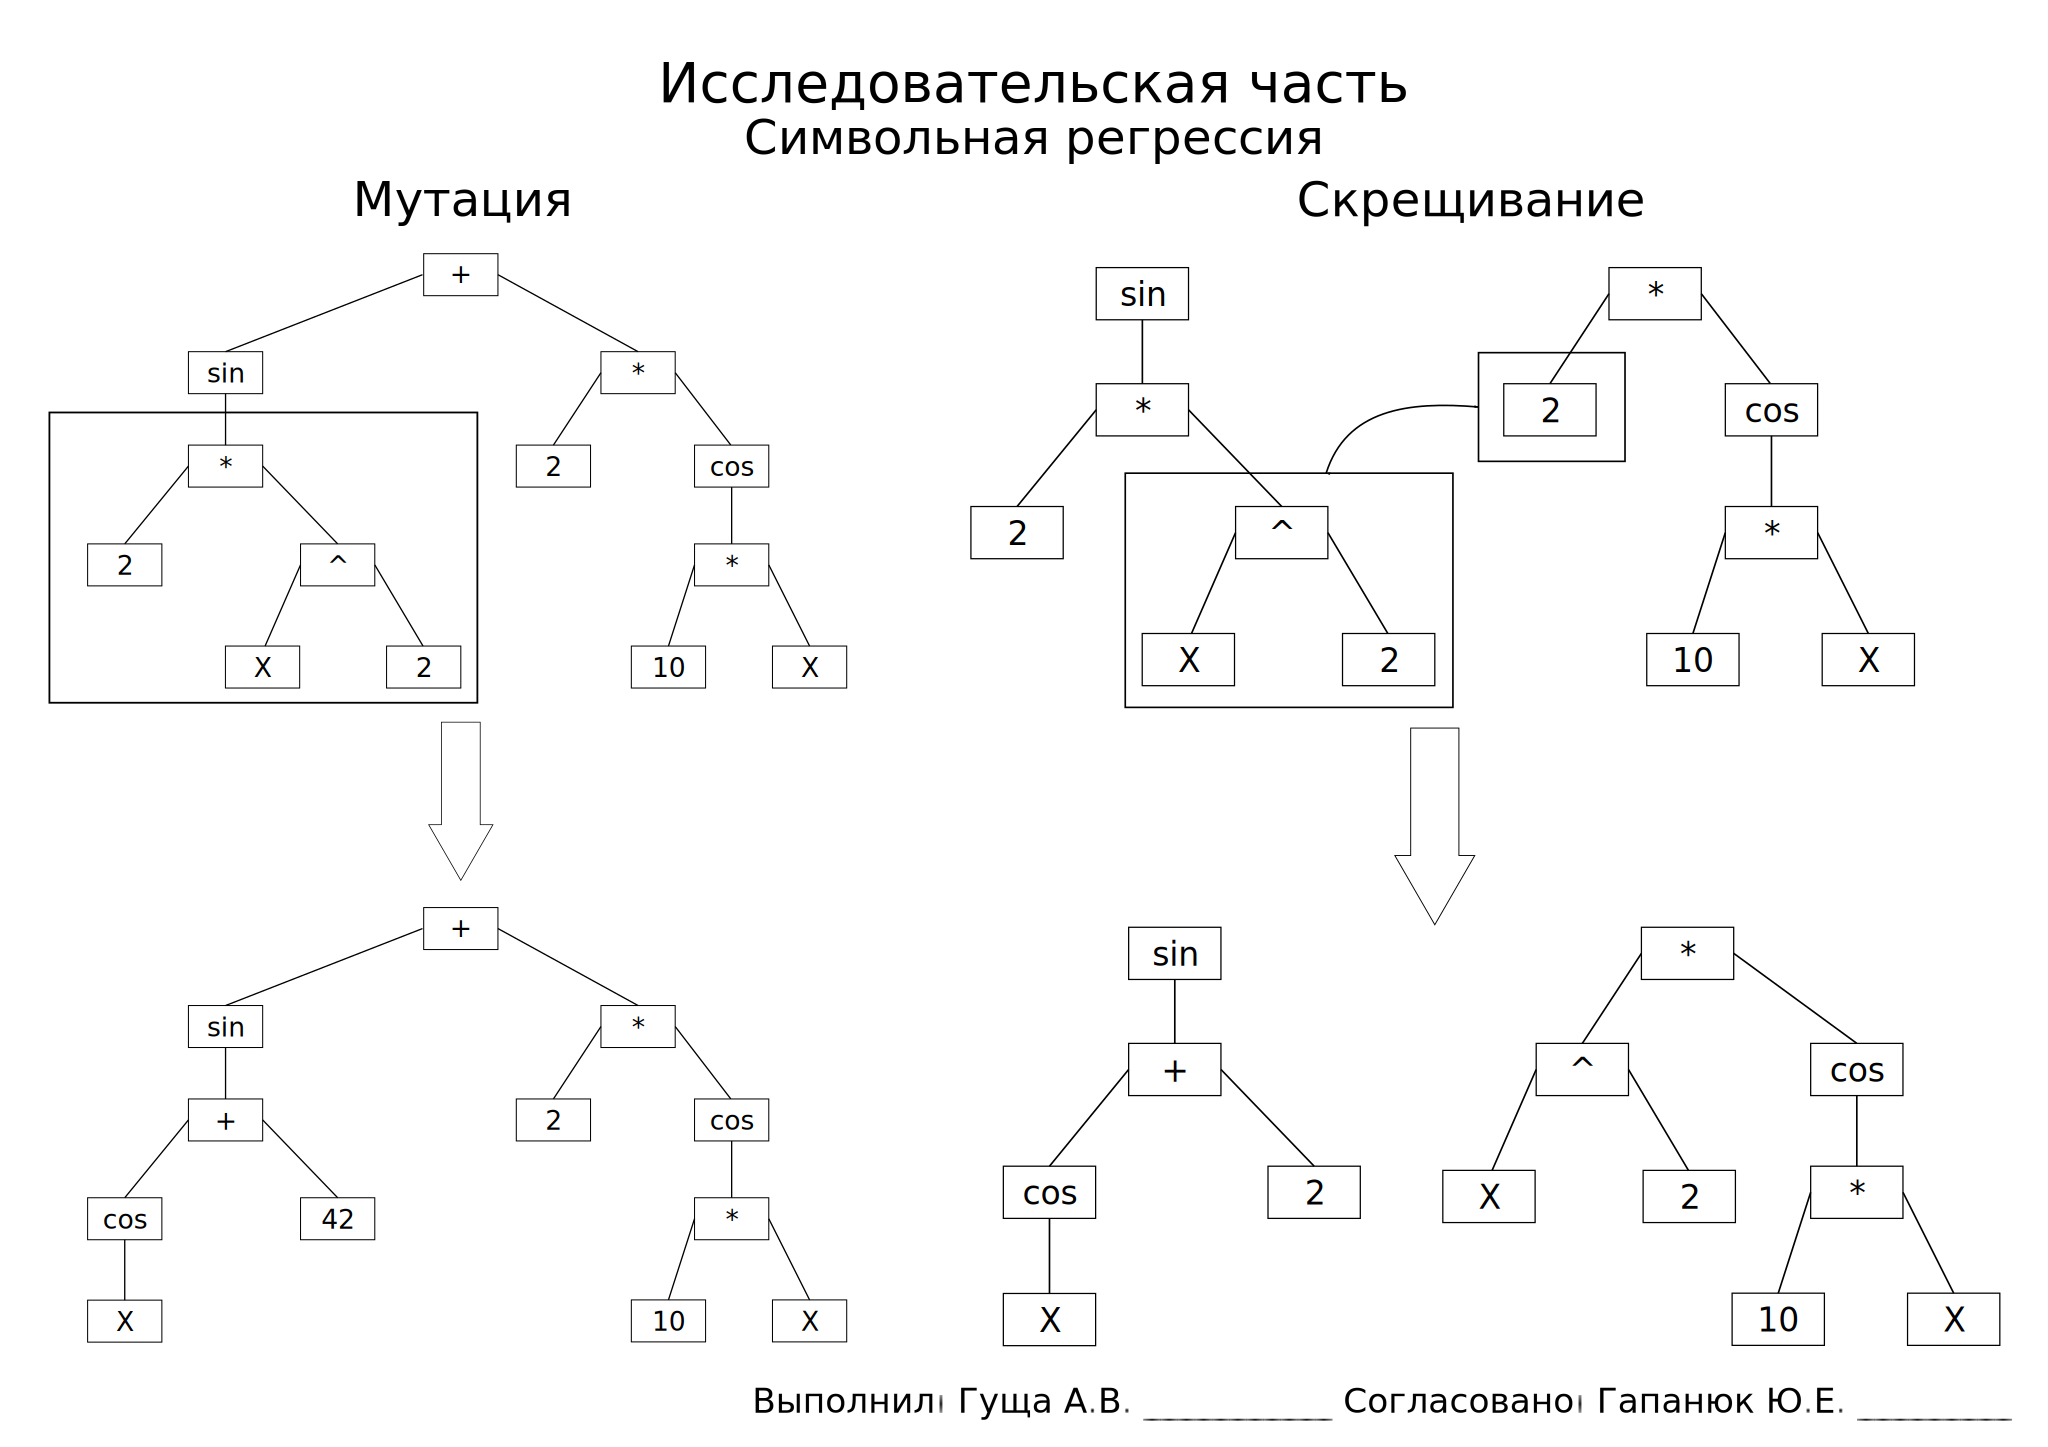
\includegraphics[width=0.90\textwidth]{lists/list10_1_2}
\end{ESKDdrawing}

\ESKDcolumnI{Основные алгоритмы}
\begin{ESKDdrawing}
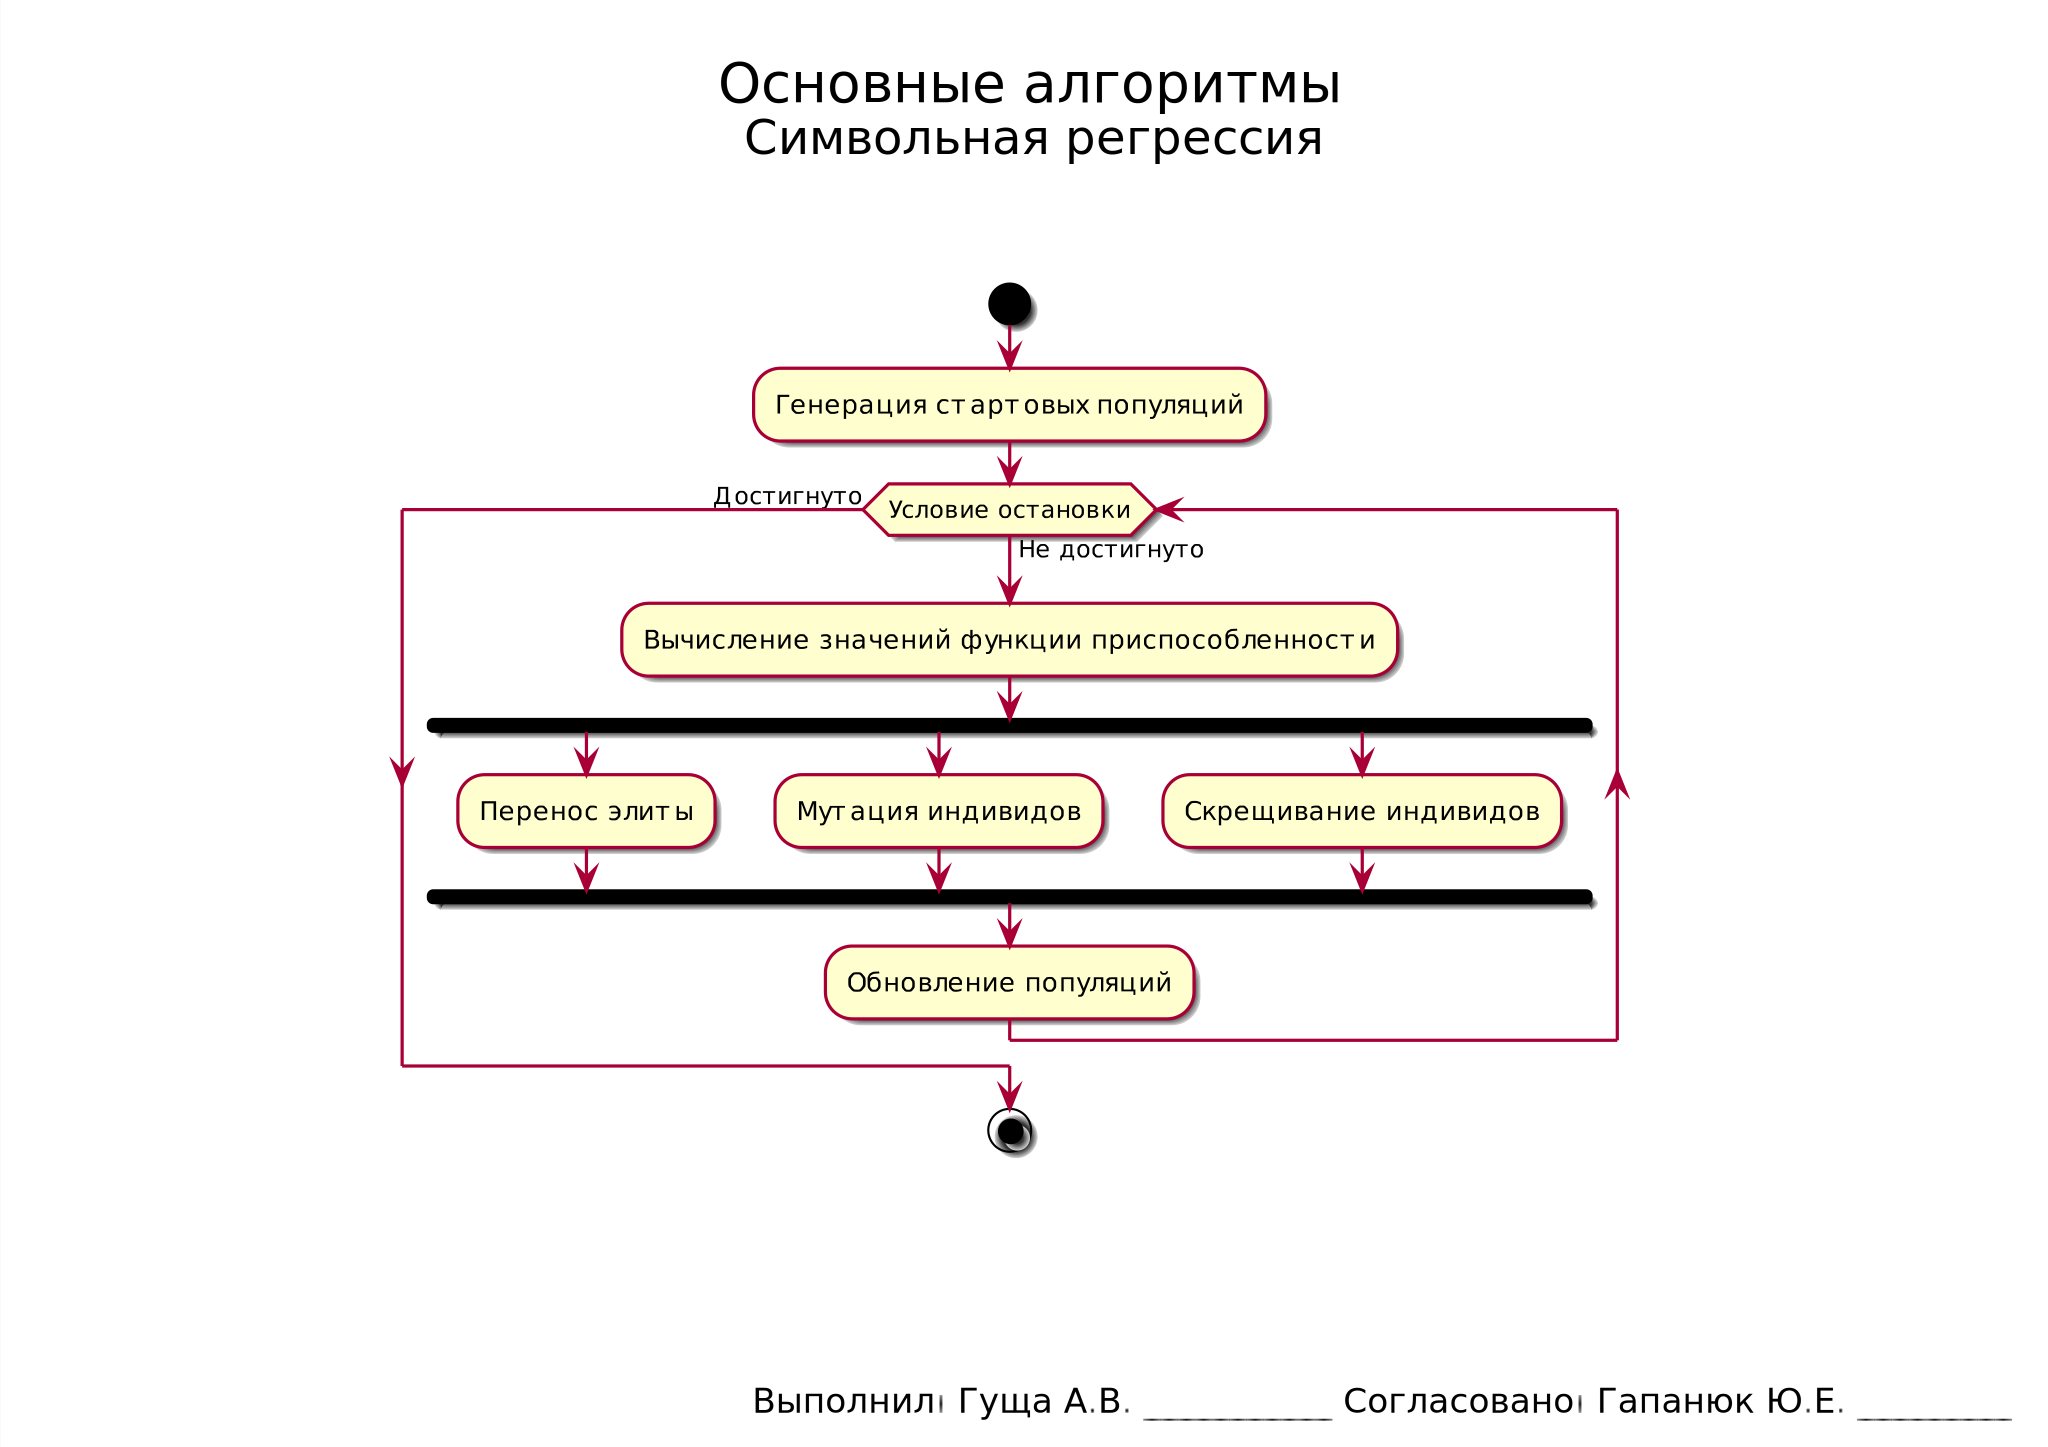
\includegraphics[width=0.90\textwidth]{lists/list11_1}
\end{ESKDdrawing}

\ESKDcolumnI{Основные алгоритмы}
\begin{ESKDdrawing}
\centering
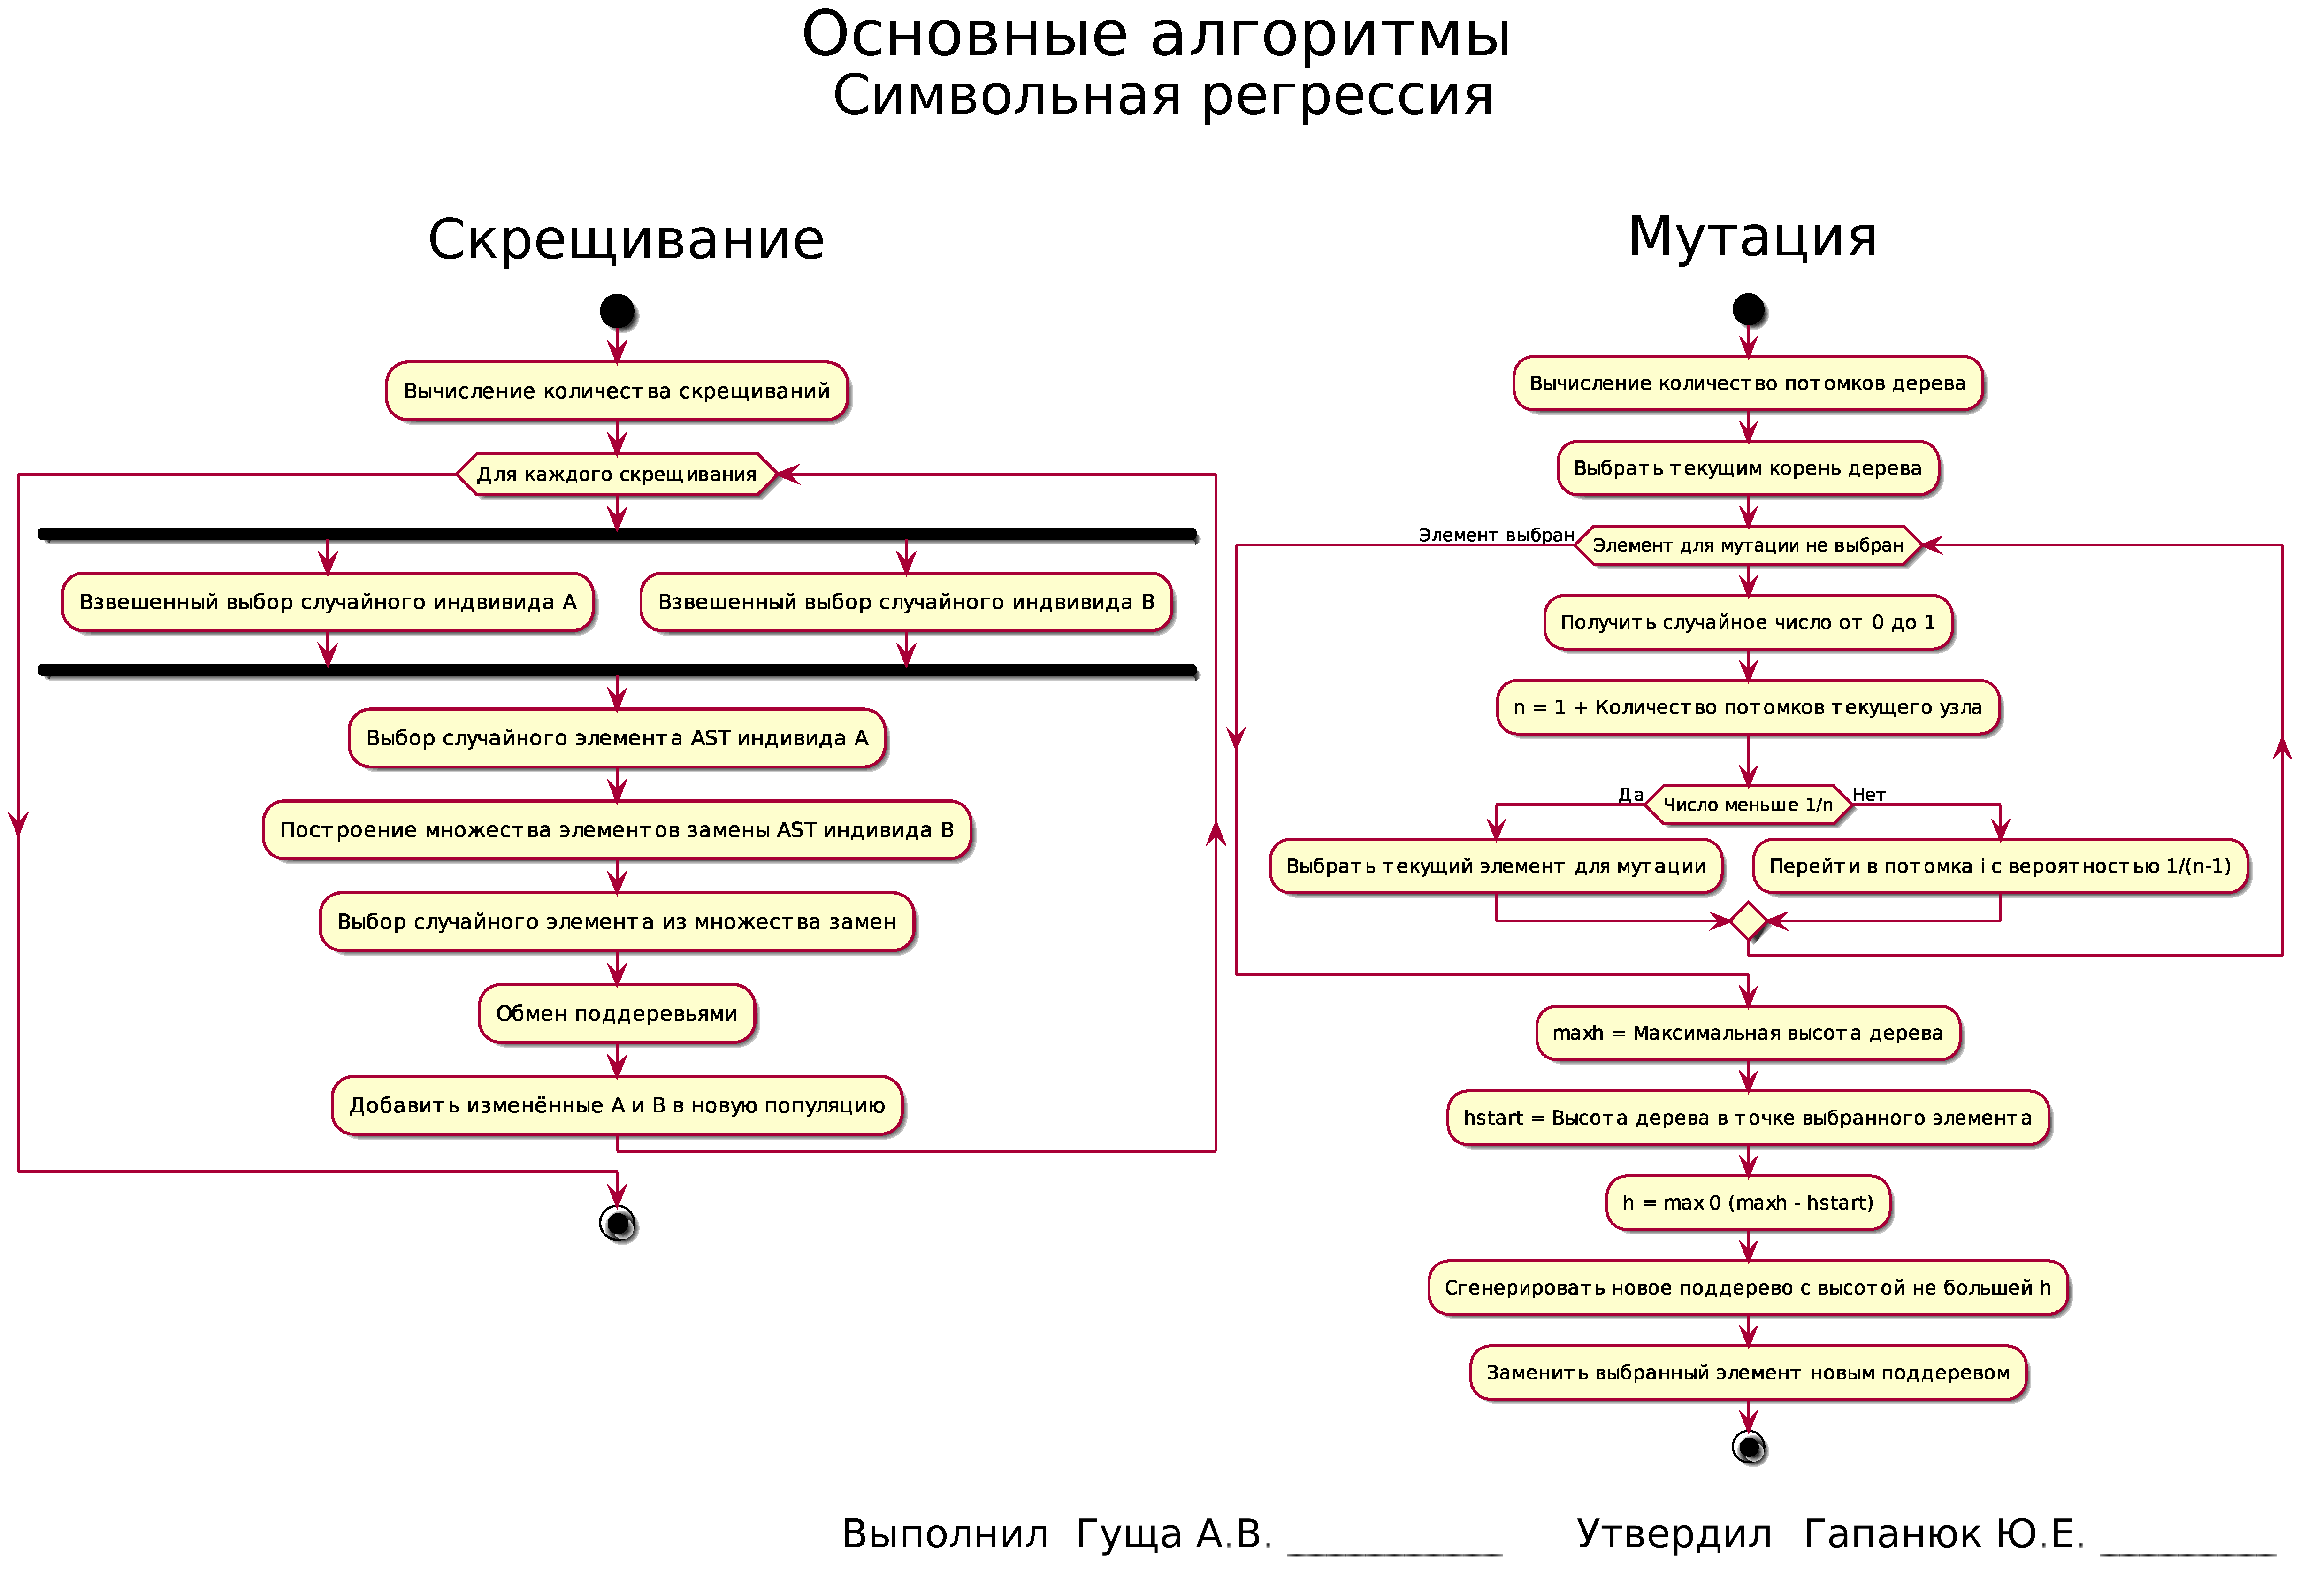
\includegraphics[width=0.90\textwidth]{lists/list11}
\end{ESKDdrawing}

\ESKDcolumnI{Исследовательская часть}
\begin{ESKDdrawing}
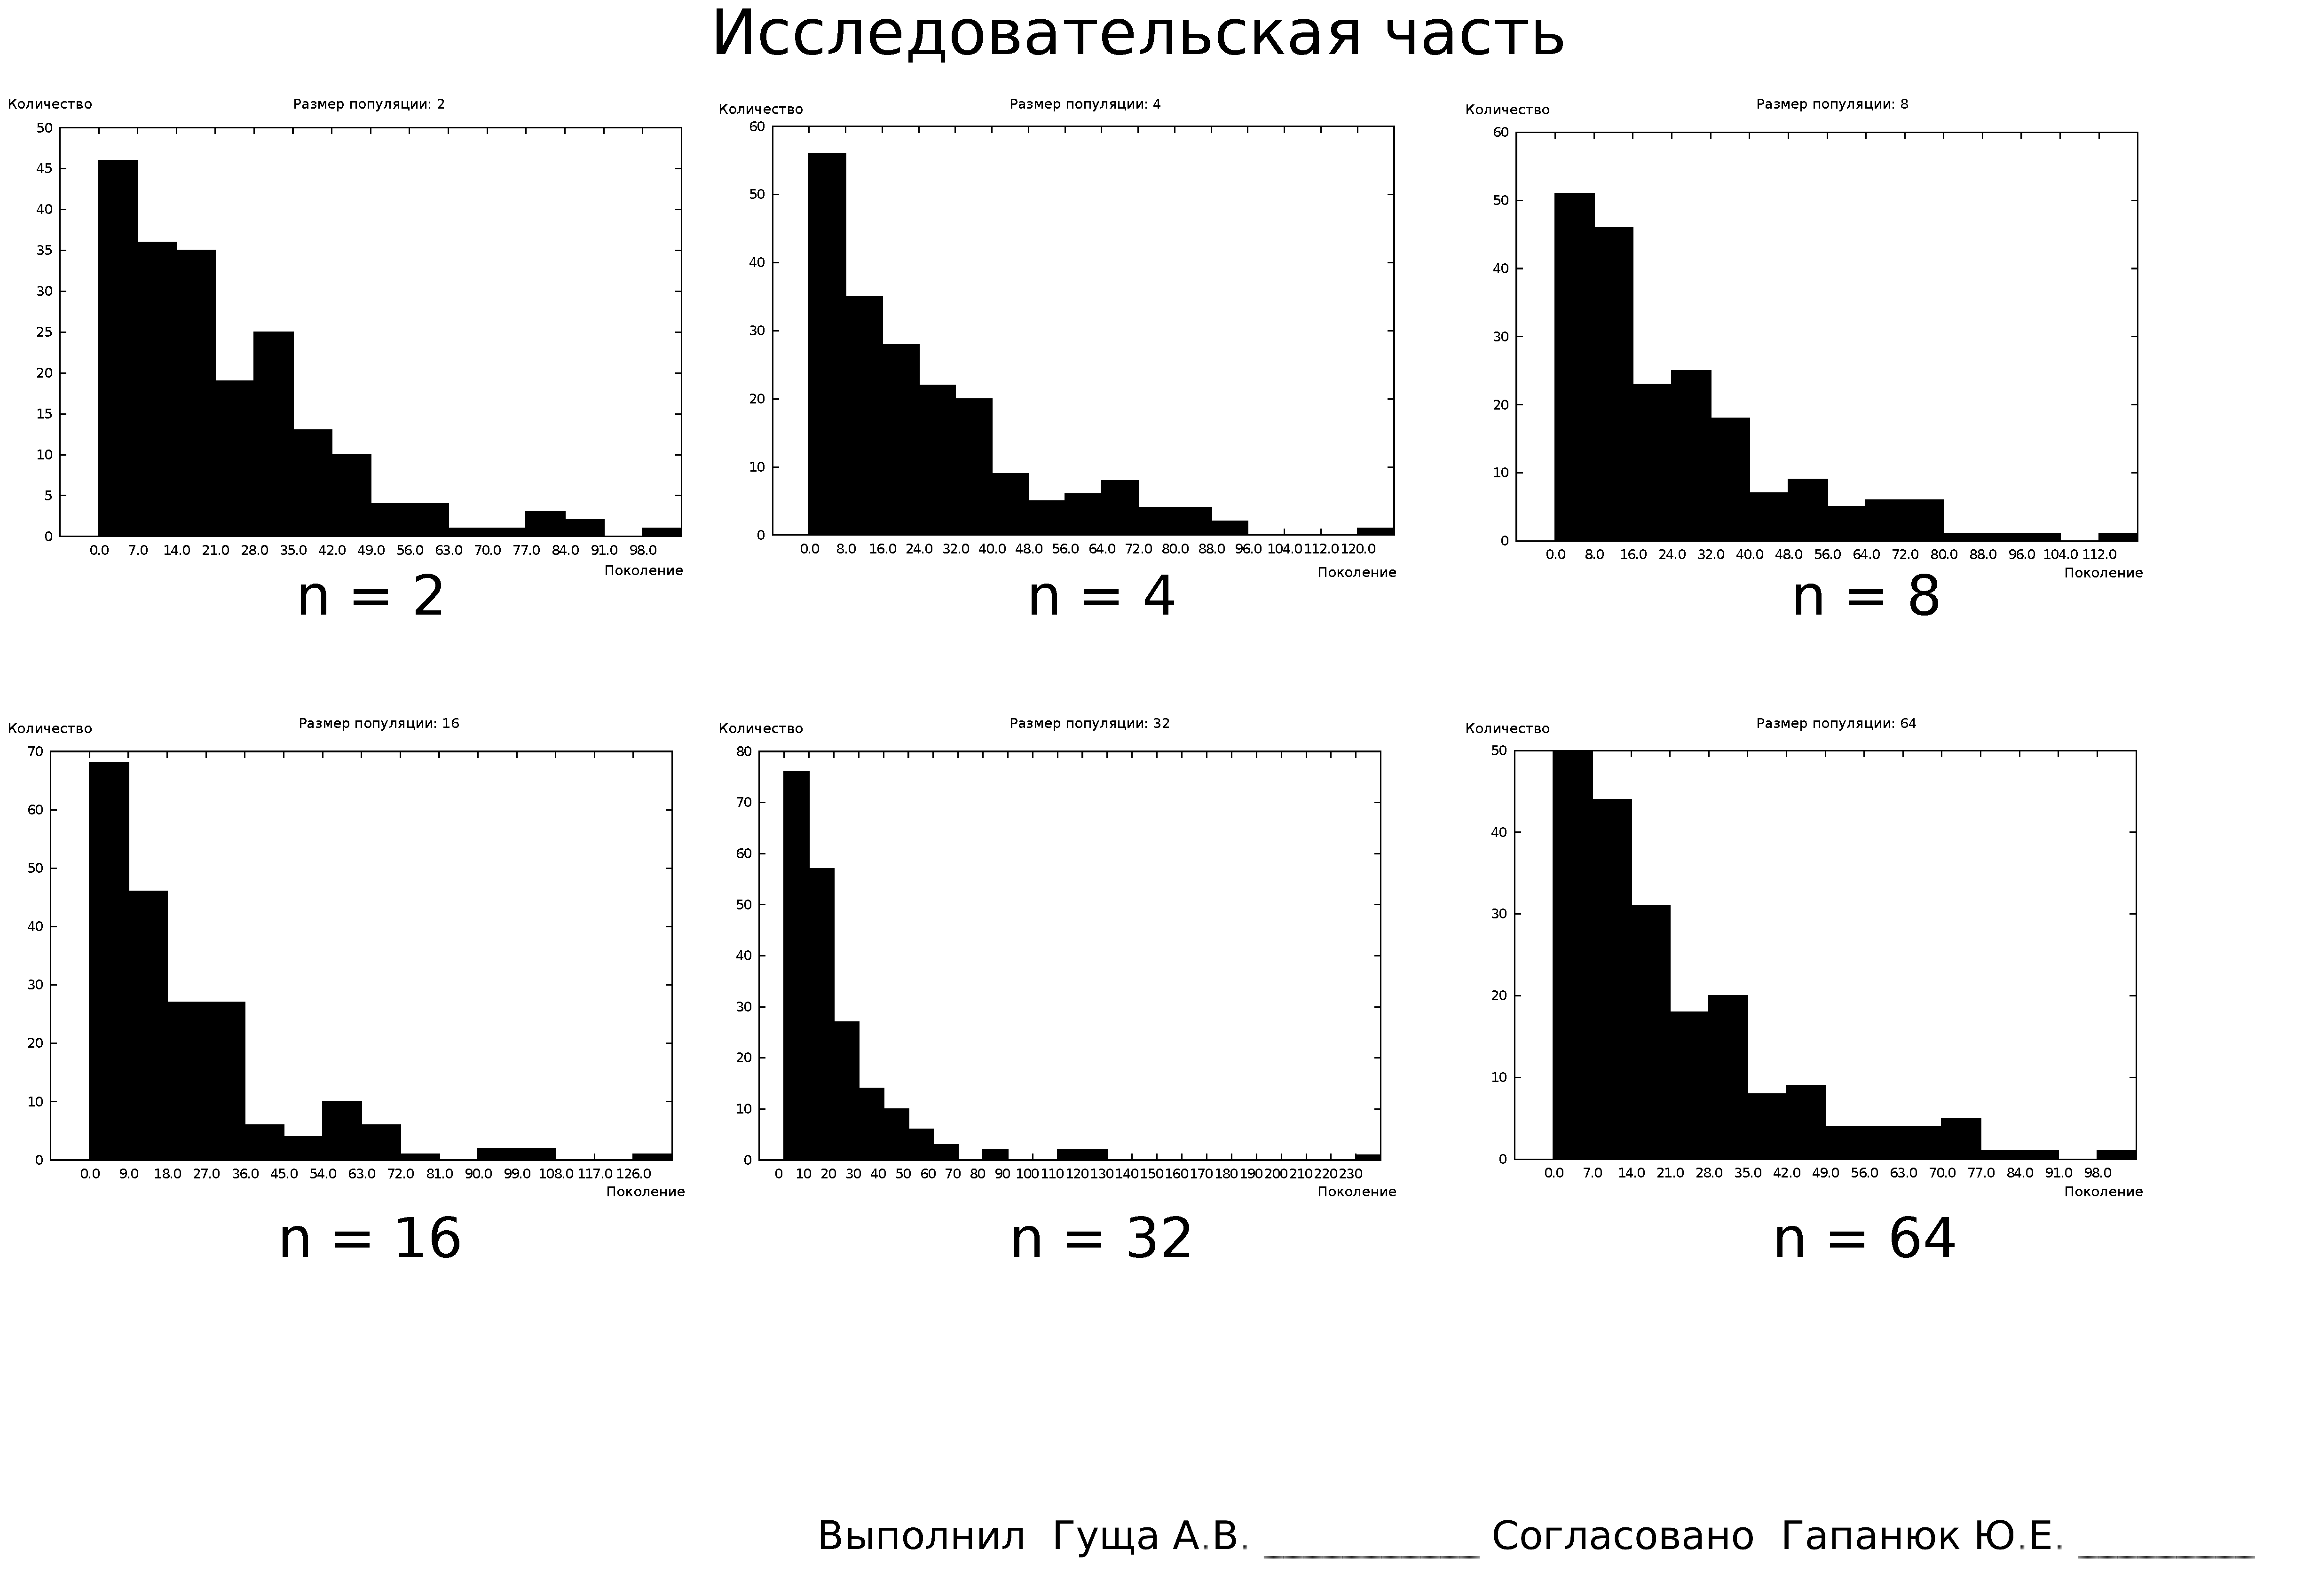
\includegraphics[width=0.90\textwidth]{lists/list10_2}
\end{ESKDdrawing}

\ESKDcolumnI{Исследовательская часть}
\begin{ESKDdrawing}
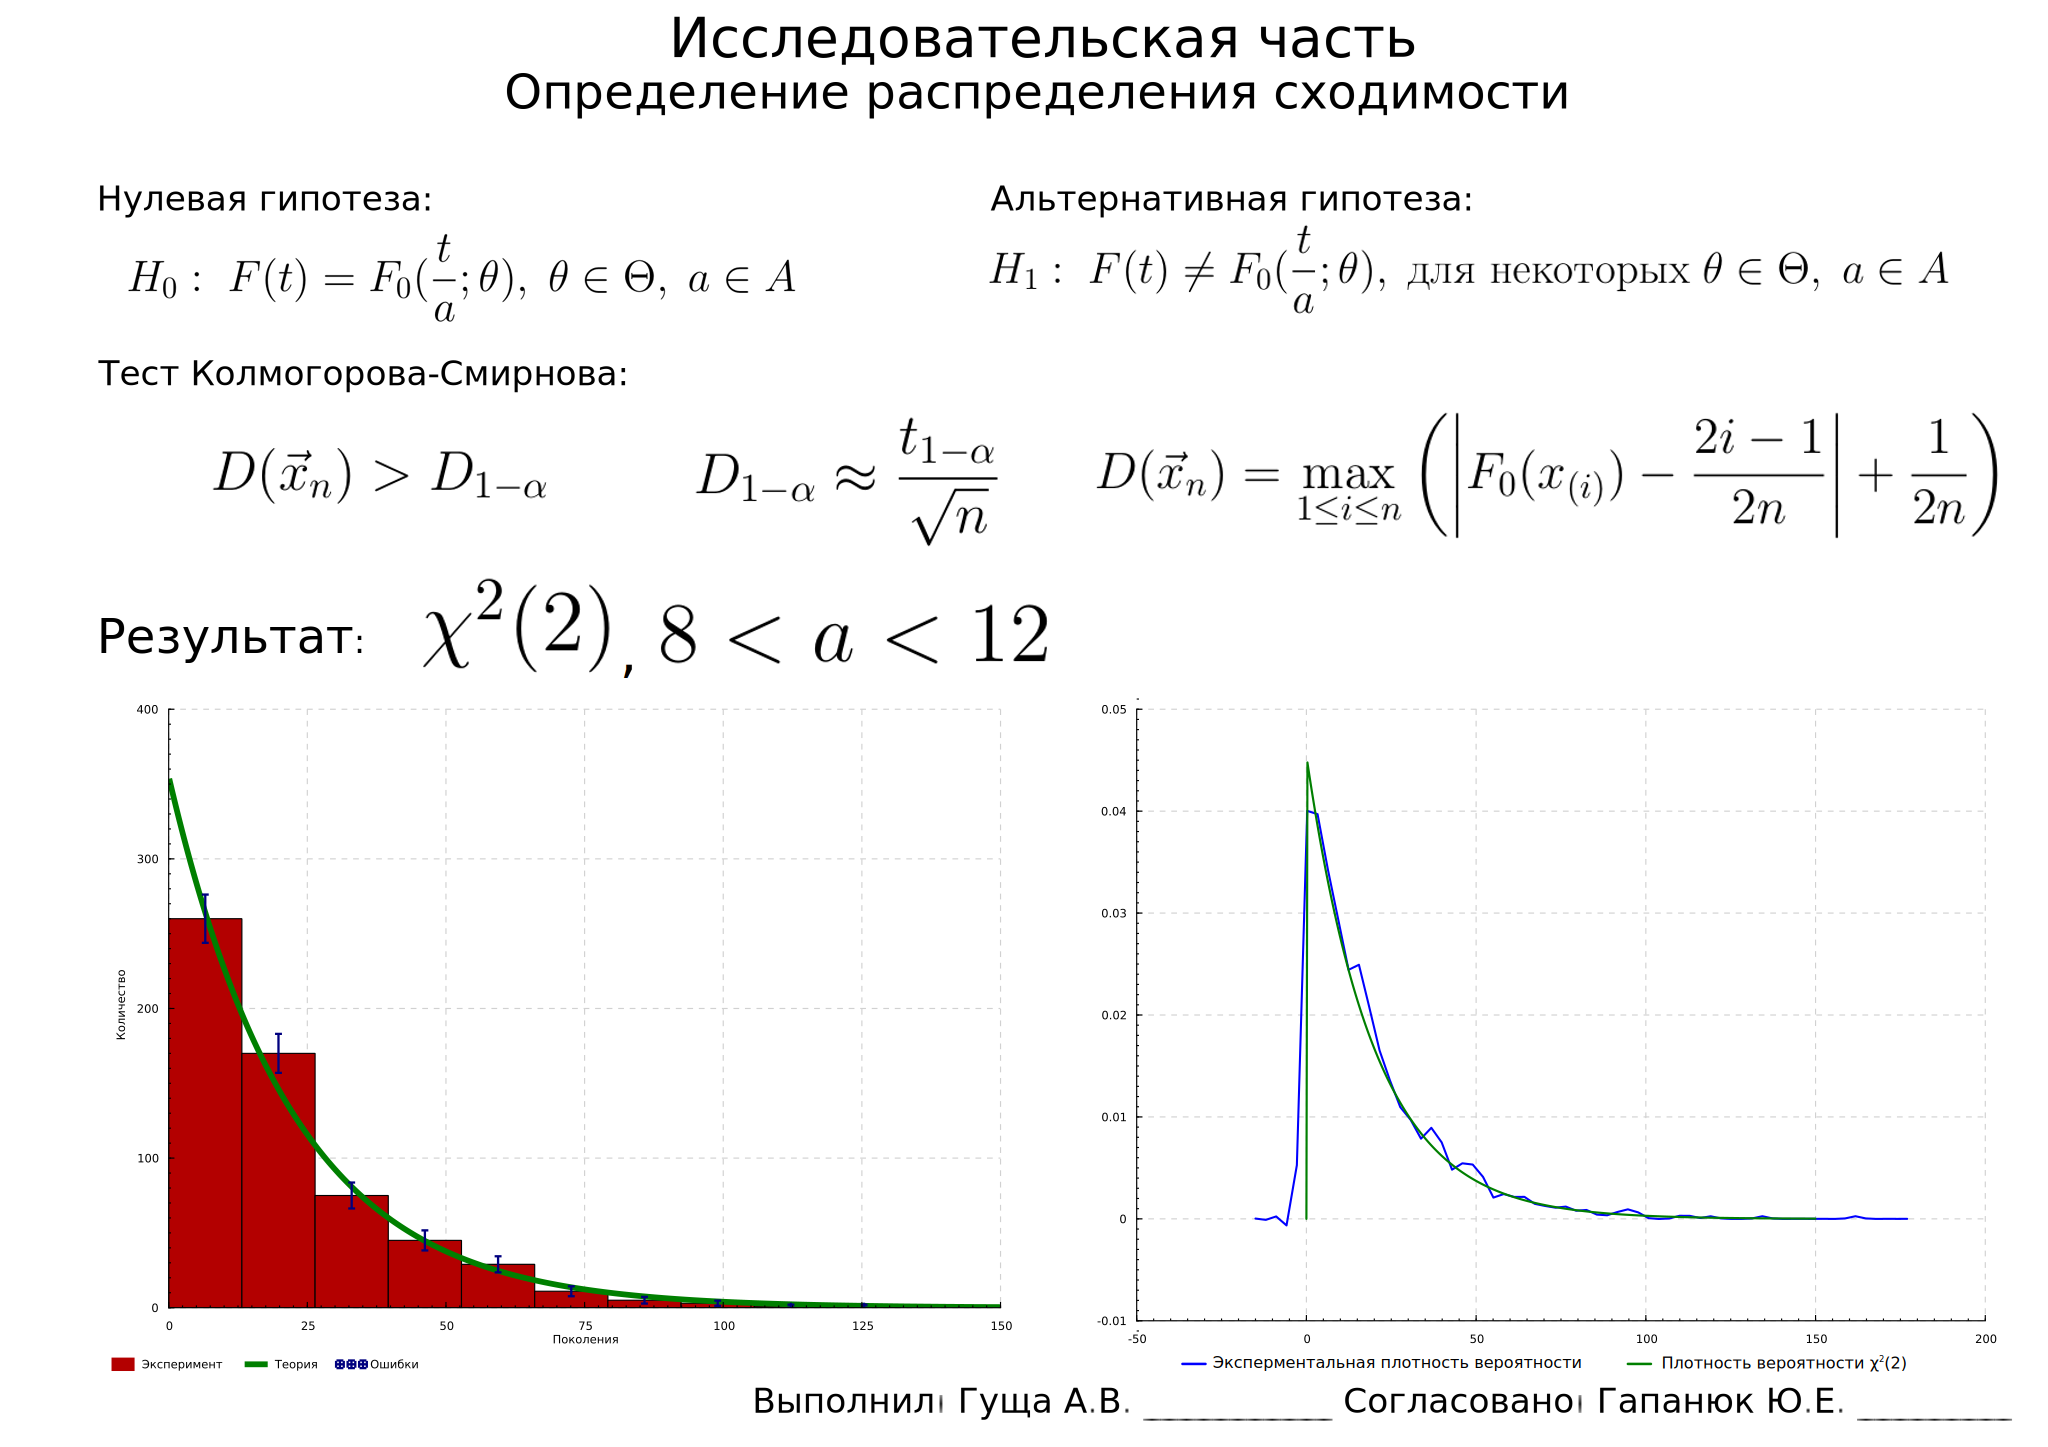
\includegraphics[width=0.90\textwidth]{lists/list10_3}
\end{ESKDdrawing}

\end{document}